% Institute of Computer Science thesis template
% authors: Sven Laur, Liina Kamm, Tõnu Tamme
% last change Eero Vainikko <eero.vainikko@ut.ee> 12.01.2021
%--
% Compilation instructions:
% 1. Choose main language on line 55-56 (English or Estonian)
% 2. Compile 1-3 times to get refences right
% pdflatex unitartucs-thesis-template
% bibtex unitartucs-thesis-template
%--
% Please use references like this:
% <text> <non-breaking-space> <cite/ref-command> <punctuation>
% This is an example~\cite{example}.

\documentclass[12pt]{article}

% A package for setting layout and margins for your thesis 
\usepackage[a4paper]{geometry}

%%=== A4 page setup ===
%\setlength{\paperwidth}{21.0cm} 
%\setlength{\paperheight}{29.7cm}
%\setlength{\textwidth}{16cm}
%\setlength{\textheight}{25cm}


% When you write in Estonian then you want to use text with right character set
% By default LaTeX does not know what to do with õäöu letters. You have to specify
% a correct input and font encoding. For that you have to Google the Web     
%
% For TexShop under MacOS X. The right lines are 
%\usepackage[applemac]{inputenc}
%\usepackage[T1]{fontenc} %Absolutely critical for *hyphenation* of words with non-ASCII letters.
%
% For Windows and Linux the right magic lines are   
% \usepackage[latin1]{inputenc}
% \usepackage[latin5]{inputenc}
%
\usepackage[utf8]{inputenc} %standard encoding since 2018 (can be commented out?)
\usepackage[T1]{fontenc} %Absolutely critical for *hyphenation* of words with non-ASCII letters.

% Typeset text in Times Roman instead of Computer Modern (EC)
\usepackage{times}

% Suggested packages:
\usepackage{microtype}  %towards typographic perfection...
\usepackage{inconsolata} %nicer font for code listings. (Use \ttfamily for lstinline bastype)


% Use package babel for English or Estonian 
% If you use Estonian make sure that Estonian hyphenation is installed 
% - hypen-estonian or eehyp packages
%
%===Choose the main language in thesis
\usepackage[estonian, english]{babel} %the thesis is in English 
%\usepackage[english, estonian]{babel} %the thesis is in Estonian

% Change Babel document elements 
\addto\captionsestonian{%
  \renewcommand{\refname}{Viidatud kirjandus}%
  \renewcommand{\appendixname}{Lisad}%
}

% If you have problems with Estonian keywords in the bibliography
%\usepackage{biblatex}
%\usepackage[backend=biber]{biblatex}
%\usepackage[style=alphabetic]{biblatex}
%% plain --> \usepackage[style=numeric]{biblatex}
%% abbrv --> \usepackage[style=numeric,firstinits=true]{biblatex}
%% unsrt --> \usepackage[style=numeric,sorting=none]{biblatex}
%% alpha --> \usepackage[style=alphabetic]{biblatex}
%\DefineBibliographyStrings{estonian}{and={ja}}
%\addbibresource{unitartucs-thesis.bib}


% General packages for math in general, theorems and symbols 
% Read ftp://ftp.ams.org/ams/doc/amsmath/short-math-guide.pdf for further information
\usepackage{amsmath} 
\usepackage{amsthm}
\usepackage{amssymb}

% Optional calligraphic fonts    
% \usepackage[mathscr]{eucal}

% Print a dot instead of colon in table or figure captions
\usepackage[labelsep=period]{caption}

% Packages for building tables and tabulars 
\usepackage{array}
\usepackage{tabu}   % Wide lines in tables
\usepackage{xspace} % Non-eatable spaces in macros

% Including graphical images and setting the figure directory
\usepackage{graphicx}
\graphicspath{{figures/}}

% Packages for getting clickable links in PDF file
%\usepackage{hyperref}
\usepackage[hidelinks]{hyperref} %hide red (blue,green) boxes around links
\usepackage[all]{hypcap}


% Packages for defining colourful text together with some colours
\usepackage{color}
\usepackage{xcolor} 
%\definecolor{dkgreen}{rgb}{0,0.6,0}
%\definecolor{gray}{rgb}{0.5,0.5,0.5}
\definecolor{mauve}{rgb}{0.58,0,0.82}


% Standard package for drawing algorithms
% Since the thesis in article format we must define \chapter for
% the package algorithm2e (otherwise obscure errors occur) 
\let\chapter\section
\usepackage[ruled, vlined, linesnumbered]{algorithm2e}

% Fix a  set of keywords which you use inside algorithms
\SetKw{True}{true}
\SetKw{False}{false}
\SetKwData{typeInt}{Int}
\SetKwData{typeRat}{Rat}
\SetKwData{Defined}{Defined}
\SetKwFunction{parseStatement}{parseStatement}


% Nice todo notes
\usepackage{todonotes}

% comments and verbatim text (code)
\usepackage{verbatim}


% Proper way to create coloured code listings
\usepackage{listings}
\lstset{ 
  %language=python,                % the language of the code
  language=C++,
  basicstyle=\footnotesize,        % the size of the fonts that are used for the code
  %numbers=left,                   % where to put the line-numbers
  %numberstyle=\footnotesize,      % the size of the fonts that are used for the line-numbers
  numberstyle=\tiny\color{gray}, 
  stepnumber=1,                    % the step between two line-numbers. If it's 1, each line 
                                   % will be numbered
  numbersep=5pt,                   % how far the line-numbers are from the code
  backgroundcolor=\color{white},   % choose the background color. You must add \usepackage{color}
  showspaces=false,                % show spaces adding particular underscores
  showstringspaces=false,          % underline spaces within strings
  showtabs=false,                  % show tabs within strings adding particular underscores
  frame = lines,
  %frame=single,                   % adds a frame around the code
  rulecolor=\color{black},		   % if not set, the frame-color may be changed on line-breaks within 
                                   % not-black text (e.g. commens (green here))
  tabsize=2,                       % sets default tabsize to 2 spaces
  captionpos=b,                    % sets the caption-position to bottom
  breaklines=true,                 % sets automatic line breaking
  breakatwhitespace=false,         % sets if automatic breaks should only happen at whitespace
  %title=\lstname,                 % show the filename of files included with \lstinputlisting;
                                   % also try caption instead of title
  keywordstyle=\color{blue},       % keywCurriculumord style
  commentstyle=\color{dkgreen},    % comment style
  stringstyle=\color{mauve},       % string literal style
  escapeinside={\%*}{*)},          % if you want to add a comment within your code
  morekeywords={*,game, fun}       % if you want to add more keywords to the set
}


% Obscure packages to write logic formulae and program semantics
% Unless you do a thesis on program semantics or static code analysis you do not need that
% http://logicmatters.net/resources/ndexamples/proofsty3.html <= writing type rules => use semantic::inference
% ftp://tug.ctan.org/tex-archive/macros/latex/contrib/semantic/semantic.pdf
\usepackage{proof}
\usepackage{semantic} 
\setlength{\inferLineSkip}{4pt}
\def\predicatebegin #1\predicateend{$\Gamma \vdash #1$}

% If you really want to draw figures in LaTeX use packages tikz or pstricks
% However, getting a corresponding illustrations is really painful  


% Define your favorite macros that you use inside the thesis 
% Name followed by non-removable space
\newcommand{\proveit}{ProveIt\xspace}

% Macros that make sure that the math mode is set
\newcommand{\typeF}[1] {\ensuremath{\mathsf{type_{#1}}}\xspace}
\newcommand{\opDiv}{\ensuremath{\backslash \mathsf{div}}\xspace} 

% Nice Todo box
\setlength{\marginparwidth}{2cm}
\newcommand{\TODO}{\todo[inline]}

% A way to define theorems and lemmata
\newtheorem{theorem}{Theorem}



%%% BEGIN DOCUMENT
\begin{document}

%===BEGIN TITLE PAGE
\thispagestyle{empty}
\begin{center}

\large
\iflanguage{english}{%
UNIVERSITY OF TARTU\\
Faculty of Science and Technology\\
Institute of Computer Science\\
Software Engineering Curriculum\\
%Software Engineering Curriculum\\
}{%\iflanguage
TARTU ÜLIKOOL\\
Loodus- ja täppisteaduste valdkond\\
Arvutiteaduse instituut\\
Informaatika õppekava\\
}%\iflanguage

%\vspace*{\stretch{5}}
\vspace{25mm}

\Large Enlik -

\vspace{4mm}

\huge Topic Modeling for Requirements Engineering: 
An Analysis of Ridesharing App Reviews 

%\vspace*{\stretch{7}}
\vspace{20mm}

\Large
\iflanguage{english}{%
Master's Thesis (30 ECTS)
}

\end{center}

\vspace{2mm}

\begin{flushright}
 {
 \setlength{\extrarowheight}{5pt}
 \begin{tabular}{r l} 
  \sffamily \iflanguage{english}{Supervisor(s)}{Juhendaja(d)}: &                    \sffamily Tahira Iqbal \\
             & \sffamily Kuldar Taveter, PhD
 \end{tabular}
 }
\end{flushright}

%\vspace*{\stretch{3}}\iflanguage
%\vspace{10mm}

\vfill
\centerline{\large Tartu \the\year}

%===END TITLE PAGE

% If the thesis is printed on both sides of the page then 
% the second page must be must be empty. Comment this out
% if you print only to one side of the page comment this out
%\newpage
%\thispagestyle{empty}    
%\phantom{Text to fill the page}
% END OF EXTRA PAGE WITHOUT NUMBER


%===COMPULSORY INFO PAGE
\newpage

%=== Info in English
\newcommand\EngInfo{{%
\selectlanguage{english}
\noindent\textbf{\large Topic Modeling for Requirements Engineering: An Analysis of Ridesharing App Reviews}

\vspace*{3ex}

\noindent\textbf{Abstract:}

\noindent
Research in AI technology has become more popular today, helped by the rising of data volumes, powerful algorithms, and easier access to high-performance computing. Natural Language Processing (NLP) as a subset of AI technology plays an important role in the future of conversational AI because of its capability to interpret our natural language. On the other hand, ridesharing app industry is growing exponentially, helped by the rise of mobile device technology and the need for faster and cheaper mobility options. In the current thesis, we provide an overview of the current industrial practices in the development of NLP applications for analyzing app reviews and identify the gap in the state-of-the-art practices. To bridge the gap, this thesis proposes a method to extract information from the app reviews, with the goal to help ridesharing app developers to identify which features are most needed and which are less important. The proposed method is compared with the other similar methods and is validated with Europe's top 10 ridesharing apps, including Bolt, Uber, Blablacar, Cabify, Via, Getaround, OlaCabs, Taxi.eu, Freenow, and Yandex Go. This contribution helps the ridesharing app developers to determine the requirements for developing their apps.

\vspace*{1ex}

\noindent\textbf{Keywords:}\\
Natural Language Processing, Data-Driven Requirements, Ridesharing, App Reviews
%Layout, formatting, template

\vspace*{1ex}

\noindent\textbf{CERCS:}\\
P170 Computer science, numerical analysis, systems, control

\vspace*{1ex}
}}%\newcommand\EngInfo

%=== Info in Estonian
\newcommand\EstInfo{{%
\selectlanguage{estonian}
\noindent\textbf{\large Teemade modelleerimine nõuete analüüsiks: sõidujagamisrakenduste arvustuste analüüs}
\vspace*{1ex}

\noindent\textbf{Lühikokkuvõte:}

\noindent
Tehisintellekti tehnoloogiate alane uurimistöö on tänapäeval muutunud populaarsemaks, millele aitavad kaasa andmemahtude kasv, kõrge jõudlusegs algoritmid ja hõlpsam juurdepääs suure jõudlusega andmetöötlusele. Loomuliku keele töötlemine osana tehisintellekti tehnoloogiatest mängib olulist roll vestluspõhise tehisintellekti tulevikus, sest suudab tõlgendada meie loomulikku keelt. Teisest küljest, sõidujagamisrakenduste tööstus kasvab plahvatuslikult, millele aitavad kaasa mobiilseadmete tehnoloogia levik ning vajadus kiiremate ja odavamate liikumisvõimaluste järele. Käesolevas magistritöös anname ülevaate tôöstuslikest sõidujagamisrakenduste arvustuste analüüsi loomuliku keele rakendustest ja selgitame välja praeguste praktikate puudujäägid. Puudujääkide leevendamiseks paneme ette meetodi teabe eraldamiseks rakenduste arvustustest eesmärgiga aidata sõidujagamisrakenduste arendajatel tuvastada, milliseid funktsioone on kõige rohkem vaja ja millised on vähem olulised. Töös võrreldakse ettepandud meetodit teiste vastavate meetoditega ja valideeritakse Euroopa kümne kõige populaarsema sõidujagamise rakendusega, kaasa arvatud Bolt, Uber, Blablacar, Cabify, Via, Getaround, OlaCabs, Taxi.eu, Freenow, ja Yandex Go.. See panus aitab sõidujagamisrakenduste arendajatel määrata kindlaks nõuded rakenduste arendamiseks.

\vspace*{1ex}

\noindent\textbf{Võtmesõnad:}\\
loomuliku keele töötlus, Andmepõhised nõuded, Sõidujagamine, Rakenduste arvustused
%Layout, formatting, template

\vspace*{1ex}

\noindent\textbf{CERCS:}\\
P170 Arvutiteadus, arvutusmeetodid, süsteemid, juhtimine (automaatjuhtimisteooria)

\vspace*{1ex}
}}%\newcommand\EstInfo


%=== Determine the order of languages on Info page
\iflanguage{english}{\EngInfo}{\EstInfo}
\newpage
\iflanguage{estonian}{\EngInfo}{\EstInfo}


\newpage
\tableofcontents

\newpage
\listoffigures

\newpage
\listoftables

\newpage
\section{Introduction}
\subsection{Motivation}
Requirements engineering as the initial phase of software engineering becomes critical to ensuring that the software development process will succeed. Requirements engineering consists of four core activities, including elicitation, documentation, validation, and management \cite{re_fundamentals}. In this thesis, we will concentrate on the elicitation activity to understand the user’s expectations from the ridesharing app. Requirements elicitation is discovering some features that our users need through several methods such as interviews, surveys, brainstorming sessions, or currently available user reviews in the app store. Elicitation using user reviews has a limitation. It can be very time-consuming to analyze a large number of user reviews if we’re doing manual analysis.

Machine learning is a branch of artificial intelligence and computer science that plays an important role in uncovering key insights from a data science project. It can imitate the way of human learning, supported by improved data quality and algorithms to make it better. There is a lot of data in the digital world today, generated not only by people but also by computers, phones, and other smart devices. These generated data will continue to grow in the coming years, as stated in Statista\footnote{\url{https://www.statista.com/statistics/871513/worldwide-data-created/}} research department. As the volume of data surpasses the ability of humans to make sense of it and manually analyze it, we will turn increasingly to the machine learning framework that can learn from the data automatically. These powerful capabilities can be applied to wide range of fields, from skin cancer detection\cite{skin_cancer_detection}, self-driving vehicles\cite{ml_for_selfdriving_car}, spam detection\cite{ml_for_spam_detection}, and many more. In correlation with this thesis, following the exponential growth of the app reviews text dataset, app developers will require machine learning to assist in identifying relevant app requirements for further app development and continuous improvement.

Natural language processing (NLP) techniques have been used in many different subjects such as language translation\cite{nlp_for_language_translation}, predictive text\cite{nlp_for_predictive_text}, sentiment analysis\cite{nlp_for_sentiment_analysis}, chatbot\cite{nlp_for_chatbot}, and many more. NLP has boosted the interest in requirement engineering (RE) research, as RE is one of the most natural language-intensive fields in the software engineering area \cite{nlp_for_re_2}. This close relationship between NLP and RE becomes the source of inspiration for researchers to seek to apply NLP techniques and tools in the step of processing requirements texts \cite{nlp_for_re}. In this past decade, NLP techniques have seen a tremendous breakthrough, especially after the development of game-changing technologies generally classified under the umbrella of deep learning \cite{trend_deep_learning_nlp}. It created stronger synergies between NLP and RE, especially with the recent widespread availability of natural language (NL) content relevant to RE, such as app reviews from users in some popular app stores.


App reviews from the two biggest mobile app platforms, Google Play Store\footnote{\url{https://play.google.com/store}} and Apple App Store\footnote{\url{https://www.apple.com/app-store/}} become one of the biggest free available sources for app developers to get users’ feedback about their mobile apps. The positive reviews can lead to more user attraction, but negative reviews can bring a sales loss. Besides that, it also can help app developers to cope with the future development plan through information like feature requests, bug reports, and user experience.

\subsection{Problem Statement}
The number of app reviews from the most popular ridesharing app, such as Uber \cite{onde}, can be massively huge, with up to 10.1 million text reviews according to the Google Play Store page of Uber app\footnote{\url{https://play.google.com/store/apps/details?id=com.ubercab}} per July 2022. Unfortunately, not all app reviews are informative and useful for app developers. App reviews in the app store are also mixed with many different languages worldwide, which will be irrelevant for those countries that only speak English, and vice versa. Some reviews also contain uninformative reviews that need to be filtered out to create high-quality input data. Analyzing this massive number of reviews with its variance will be time-consuming and very difficult to process, possibly being error-prone for app developers.

\subsection{Objectives}
The main objective of this thesis is to create an analysis report based on the ridesharing app reviews that will be useful for the app developer in the purpose of getting to know what their customer wants with their app. The scope of this thesis project is currently focused only on the field of ridesharing apps.

To avoid the manual approach, which is time-consuming, we are applying some automation approaches based on the NLP approaches using Python programming language and its supporting libraries. Getting started with some open-source projects, we’re doing the preprocessing steps, such as removing non-English reviews, filtering out inconsistent and uninformative reviews, and applying topic modeling to analyze the app reviews.

\newpage
\subsection{Research Questions}
Based on the problems mentioned in the previous section, we formulated the following two research questions (RQs) to guide our research.
\begin{itemize}
\item \textbf{RQ1}: What kind of NLP approaches are more effective for automatic app review classification?

Many different NLP approaches are currently available. We will focus only on the approaches that are available as open-source projects and have good documentation.


Answering RQ1 involves: 
\begin{itemize}
\item Comparing the performance of different NLP approaches and currently widely used Pre-Trained Models (PTM) for NLP research
\end{itemize}

\item \textbf{RQ2}: What topics should the app developer focus on based on the analysis of topic proportion with its average rating and sentiment scores?

Using topic proportion, average ratings, and sentiment scores, we can measure each topic's performance and create the "most important topics" report based on these results.

Answering RQ2 involves:
\begin{itemize}
\item Analyzing the proportion of topics across all top-10 ridesharing apps
\item Comparing the average rating and sentiment scores for each topic per each ridesharing app, in order to get the most important topics that need to be focused on
\end{itemize}
\end{itemize}


\subsection{Contribution}
This thesis work will contribute to creating a text analysis for ridesharing app reviews which will help the app developer to use this analysis for future development in the domain of ridesharing apps. The proposed approach used 100,000+ app reviews from Europe's top 10 ridesharing apps.


\subsection{Outline of the Thesis}
The thesis is structured into three main chapters with the conclusion, references, and appendices. The remainder of the thesis is structured as follows. Chapter 2, \textbf{Literature Review}, discusses some related works of literature to this thesis. Chapter 3, \textbf{Study Setup}, describes a detailed description of the analysis process, starting from how we choose the top ten ridesharing apps in Europe, data preprocessing, and building the text corpus for the following data analysis. Chapter 4, \textbf{Implementation}, explains our proposed topic modeling techniques. Chapter 5, \textbf{Findings and Analysis}, reports on the findings and analysis for our project. Chapter 6, \textbf{Conclusion}, discusses the key results, limitations, and future work for this thesis. For the last two chapters, \textbf{References}, include related works of literature and articles, and \textbf{Appendices}, stated all the necessary information that becomes a part of this thesis project.



\newpage
\section{Literature Review} 
In the past few years, researchers have proposed many new approaches to extract features from app reviews with different methodologies automatically. However, some limitations prevent app developer teams from using the information in the app reviews. First, app stores have a large number of app reviews, which require a considerable effort to analyzing them. Second, the quality of app reviews varies widely, from helpful suggestions and ideas for app development to emotional comments. Third, one review usually contains a mix of sentiments, which makes it harder to filter positive, neutral, and negative feedback. In this chapter, we discussed some literature in the field of app review analysis that tried to tackle some of these limitations.

Guzman et al. \cite{fine_grained} proposed an automated approach to identify fine-grained features in the app reviews, then give the sentiment scores from the identified features, and use LDA topic modeling techniques to group these features into more meaningful high-level features. The data source includes 32210 app reviews from seven apps as the training data and 2800 manually peer-analyzed app reviews as the test data. Using Collocation Finding Algorithm to get the collection of words, SentiStrength to get sentiment scores, and LDA topic modeling to group several features into a set of words that construct a topic. The result stated that feature extraction has high precision results for apps with short reviews (simply praise or dispraise). They also found that their approach works well for all app categories except games and high precision results for apps with short reviews.

Di Sorbo et al. \cite{surf} identified the difficulty with manual analysis by the app developer when it has a massive amount of app review data and the unstructured nature of their content. Their data sources comprised 2622 app reviews, mined from three different app stores and relating to 12 apps. They propose SURF (Summarizer of User Reviews Feedback)  to extract specific topics and then group each app review according to its topic with a report in XML format.

The study of Rekanar et al. \cite{sentiment_analysis_hse_ireland} tried to find out the issue of the ineffectiveness of the digital contract tracing app to be aware of user concerns. Using 1287 app reviews from Google Play Store and Apple App Store of the Irish HSE COVID-19 contact tracing app, they analyzed the sentiment analysis to classify positive, negative, and neutral sentiment from each app review. They used manual analysis because the precision and recall value from the current automated sentiment analysis is still not good enough for their research. Another reason is that the total number of analyzed app reviews is not huge and is suitable for manual analysis. The final result is that most of the negative comments were aimed at the app’s performance and usability.

The study by Binkhonain and Liping Zhao \cite{review_ml} compared 24 related papers related to machine learning (ML) algorithms for identification and classification purposes. Of the 24 selected papers, only 20 have reported their performance measures. There are a total of 16 different ML algorithms, categorized into seven supervised learning (SL), four unsupervised learning (USL), and five semi-supervised learning (SSL). Rule-Based (RB) has the highest precision scores, but only one study reported this algorithm. Support Vector Machines (SVM), Naive Bayes (NB), and Decision Tree (DT) have multiple reports from different studies, but their performance varies from study to study. The result showed that supervised learning (SL), such as SVM and NB, performed better than unsupervised learning (SSL), such as Latent Dirichlet Allocation (LDA) and K-means. Their study stated that SVM and NB have the best performance, while SVM became the most frequently used algorithm. ML algorithms perform better when features are created with individual words instead of phrases. The best result was also achieved when the original word was used before stemming, or lemmatization pre-process. To tackle some challenges in the implementation of ML algorithms for Requirements Engineering (RE) purposes, the author suggested the creation of shared datasets in order to take full advantage of supervised ML algorithms. Moreover, for better result in comparison and also calling for the close collaboration between RE and ML communities to address many challenges in the development of real-world applications of ML to RE.

The study of Shah et al. \cite{faiz_ali} combined the existing app review classification model with app feature extraction techniques to develop the tool named REVSUM to extract information from app reviews for future software maintenance and release planning activities. The author also prepared the labeled review dataset from previous studies in order to help to train the new model. It stated that having annotated app reviews in the training data will improve recall scores at the cost of a drop in precision.

The study of Jung Akim \cite{jung_kim} utilized 12,566 Netflix app reviews from the Amazon app store and compared the classification result from LDA Topic Modeling and BERT Pre-Trained ML model. They found that LDA model works well for app reviews with similar keywords, while BERT model is sensitive to sentiments, especially sarcastic reviews. Both approaches have only 43\% classification agreement with 6,283 unseen reviews, and BERT occasionally works better to detect sarcasm reviews.

The SAFE approach proposed by Johann et al. \cite{safe_paper} is a simple rule-based approach to extract and match the app features from both app descriptions and app reviews. The authors did a manual analysis of app descriptions from 10 apps in the Apple App Store and identified the most frequent text patterns used to tag each app's features. For the evaluation, the author used a random sample of 5000 app reviews for each app. SAFE first apply some text preprocessing steps, including filtering three types of sentences: URL, email address, and quotations. Then, word-tokenizes each sentence and attach a POS (part-of-speech) tag to each token. For the feature matching, SAFE used the synonym sets of the words. For example, "take photo" and "capture image" is a match. Regarding the study result, SAFE significantly improved precision and recall scores compared to the previous study. Despite the encouraging results, we will need a machine learning approach for the future improvement of SAFE.

SIMBA (SIMilarity Based Approach) from Oehri et al. \cite{simba_paper} is a fine-grained approach for identifying and measuring similarity between feedback across different platforms and languages. Their dataset comprised 464,330 app reviews across four platforms: Google Play, App Store, Twitter, and Facebook. A total of 4,100 manually annotated reviews by two annotators were used for the evaluation process. SIMBA has a translation step for non-English app reviews before transforming it into the preprocessing steps. It combines currently available approaches such as NLP, lexical sentiment analysis, and supervised ML. For the classification in SIMBA, the authors used Multinomial Naive Bayes (MNB) and divided it into three categories: “feature request”, “bug report", and “other.” The results showed that SIMBA had a 79\% average correlation with manually annotated app reviews, which indicated a strong positive correlation with human annotation. Regarding future improvement, the authors mentioned adding lexical databases to handle common slang words in app reviews and creating ML models from a more diverse dataset on different platforms.

\begin{table}
\caption{Overview of Literature Review Including its Dataset, Methodology, and Result}
\begin{tabular}{|p{2cm}|p{2cm}|p{4cm}|p{5cm}|}
\hline
\centering
Paper Name & Dataset & Methodology & Result \\
\hline
A Fine Grained Sentiment Analysis of App Reviews \cite{fine_grained}
& 
\textbf{Traning data:}
\newline
total 32,210 reviews from 7 apps (Apple App Store and Google Play Store)
\newline

\textbf{Test data: }
\newline
2800 manually peer-analyzed reviews
& 
\textbf{Collocation Finding Algorithm}\newline
Collection of words that co-occur unusually often
\newline\newline
\textbf{SentiStrength}\newline
Lexical sentiment extraction tool
\newline\newline
\textbf{LDA Topic Modelling}\newline
Grouping several different features into a set of words
&
\textbf{Feature Extraction}\newline
Works well for all app categories except games (AngryBird), with the possible explanation that game app features can be described in different ways.\newline
High precision results for apps with short reviews (usually only include praise or dispraise), as it will be filtered by this automated approach to help app developers focus on the more informative reviews.
\newline\newline
\textbf{Sentiment Analysis}\newline
Strong positive correlation between the sentiment score and truth set sentiment score
\\
\hline
SURF: Summarizer of User Reviews Feedback \cite{surf}
&
2622 app reviews, mined from 3 different app stores and relating to 12 apps
&
\textbf{SURF tool for analyze large amount of app reviews:}

Extract the specific topics (e.g., UI improvements, security/licensing issues, etc.);

Identify the specific task (e.g., bug fixing, feature enchancement, etc.);

Present the result in the form of a condensed, interactive, and structured agenda of recommended software changes
&
Output report in XML format;

Can be filtered along a two-level hierarchy:
\begin{enumerate}
    \item the sentences are grouped together according their topics (e.g., App, GUI, etc.)
    \item sentences in each topic are grouped by intention categories, which were assigned during the intention classification step
\end{enumerate}
\end{tabular}
\hline
\label{tab:literature_review}
\end{table}


\begin{table}
\begin{tabular}{|p{2cm}|p{2cm}|p{4cm}|p{5cm}|}
\hline
\centering
Sentiment analysis of user feedback on the HSE’s Covid-19 contact tracing app \cite{sentiment_analysis_hse_ireland}
&
1287 user reviews from Google Play Store / Apple App Store of Irish HSE Contact Tracker app
&
Manual analysis because the precision and recall rates from current automated sentiment analysis are still not perfect
&
Classification of the issues (Pillar);
\newline
Positive / Neutral / Negative sentiment;
\newline
Review Segment;
\newline
Most of negative comments were aimed at a performance and usability
\\
\hline
A review of machine learning algorithms for identification and classification of non-functional requirements \cite{review_ml}
&
Using Wohline's snowballing method to listing down the papers required for this research;
\newline\newline
\textbf{24 related papers}:
IEEEXplore (10 papers)\newline
Springer Link (8 papers)\newline 
Science Direct (3 papers)\newline
ACM Digital Library (2 papers)\newline
Semantic Scholar (1 paper)
&
\textbf{Snowballing approach}
alternative to the traditional systematic literature review (SLR) approach;\newline
Backward snowballing (looking at the reference list of a paper);\newline
Forward snowballing (looking at the citations in which the paper is actually cited)\newline\newline
\textbf{Extracting and Synthesizing the data}\newline
extract seven data items from each paper;\newline
using constant comparison method (CCM) and summarization for qualitative analysis and synthesizing the extracted data;
&
\textbf{RQ1:}\newline
16 different ML algorithms from 24 selected papers, categorized into: 7 supervised learning, 4 unsupervised learning, 5 semi-supervised learning (SSL)\newline

\textbf{RQ2:}\newline
Revealed a general process pattern for applying ML-based approach, divided into 3 major phases: the text preparation phase, the learning phase, the evaluation phase\newline

\textbf{RQ3:}\newline
From 24 selected papers, only 20 of them have reported their performance measures\newline


\textbf{Key Findings}:\newline
ML-based approaches give more than 70\% accuracy;\newline
Overall, SL perform better than USL;\newline
ML algorithms produce the best result when using original word, instead of stemming and lemmatization

\end{tabular}
\hline
\end{table}


\begin{table}
\begin{tabular}{|p{2cm}|p{2cm}|p{4cm}|p{5cm}|}
\hline
\centering
Extracting information from app reviews to facilitate software development activities \cite{faiz_ali}
&
\textbf{SHAH dataset:}\newline
labeled review dataset belonging to different app categories;\newline\newline
review datasets along with the annotation guidelines (AGs) from previous studies\newline
&
\textbf{REVSUM:}\newline
Combined review classification and automatic feature extraction methods\newline\newline
\textbf{Review Classification Model:}\newline
Indicate that the traditional classification model (using Bag of Words features) gave result that can be competed with deep learning model
&
Using the context information from the previous or next sentences of app review can improve the performance of classification models\newline\newline
\textbf{App Feature Extraction:}\newline
SAFE has high recall, low precision - Supervised CRF (Conditional Random Field) model has high precision, low recall (opposite of SAFE);\newline
Having annotated app reviews in the training set enables to improve recall at the cost of the drop in precision\newline

\textbf{Competitive Analysis:}\newline
REVSUM, as useful tool for information extraction to be used for software maintenance and release planning activities
\\
\hline
Netflix App review Topic Modeling \cite{jung_kim}
&
12,566 app reviews from Netflix app in Amazon App Store
&
LDA Topic Modeling\newline

BERT Pre-Trained Model
&
LDA-Mallet and BERT have only 43\% classification agreement with 6,283 unseen reviews.

LDA topic model works well with reviews that have words that are coherent with the context. Not working very well with sarcastic reviews.

BERT model occasionally works better when detecting sarcastic reviews.
\end{tabular}
\hline
\end{table}


\begin{table}
\begin{tabular}{|p{2cm}|p{2cm}|p{4cm}|p{5cm}|}
\hline
\centering
SAFE: A Simple Approach for Feature Extraction from App Descriptions and App Reviews \cite{safe_paper}
&
App descriptions and reviews of 10 apps in category “productivity” from the Apple App Store.\newline

For the evaluation, a random sample of 5000 reviews for each app
&
\textbf{Text Preprocessing}\newline
Filters 3 types of sentences: sentences contain URL, email address, and quotations; bullet points and multiple symbols are removed; word-tokenizes each sentence and attach POS (part-of-speech) tags to each word token.
\newline
\newline
\textbf{Application of SAFE pattern}\newline
Analyze and decompose sentence; extract raw features; remove duplicate and noise;
&
\textbf{Feature Extraction from App Descriptions}
Based on 10 apps and 197 features (~20 per app), they got overall average precision of 55.9\% and a recall of 43.4\%
\newline\newline
\textbf{Feature Extraction from the App Reviews}
Recall of 70.9\% and precision of 23.9\%
\newline\newline
\textbf{Matching Features in the Descriptions and the Reviews}
Recall of 56\% and precision of 70.4\%
\\
\hline
Same Same but Different: Finding Similar User Feedback Across Multiple Platforms and Languages \cite{simba_paper}
&
464,330 user feedback entities from four different platforms, for a duration timespan of 60 days.
\newline\newline
4,100 manually annotated feedback.
&
SIMBA (SIMilarity Based Ap-
proach), a fine-grained approach for identifying and measuring
similarities between feedback written across different plat-
forms and languages.
\newline\newline
Combine some approaches such as automatic machine translation, NLP, lexical sentiment analysis, and supervised ML.

&
SIMBA strongly correlates to human judgment, with an average correlation of 79\% for cross-platform user feedback written in English and 78\% in four different languages.
\newline\newline
SIMBA works slightly better on longer feedback than on
feedback samples including feedback of less that five words.
\\
\end{tabular}
\hline
\end{table}

% \clearpage
% \newpage
Table \ref{tab:literature_review} provides the summary of the research papers we have discussed, including their dataset, methodology, and the result. The most used domain in these research papers is the popular mobile apps in the App Store, such as Netflix for entertainment, Whatsapp for communication, and TripAdvisor for travel. By implementing different ML algorithms, these papers are trying to extract information from app reviews automatically while also measuring their performance result. Support Vector Machines (SVM) and Naive Bayes (NB) are the best two ML algorithms discussed in many studies. SVM and NB also give the best result in terms of precision and recall score.

After reviewing some related works above, we have found some research gaps that we want to explore in this thesis. Even though many different mobile app categories have been discussed, the domain ridesharing app category has not become the main focus of these researches. Short reviews that only include praise or dispraise (for example: “I love it,” “I hate this app”) according to Guzman et al. \cite{fine_grained}, gave no information for analysis, which will be handled in this thesis in the NLP preprocessing steps. Manual review by Rekanar et al. \cite{sentiment_analysis_hse_ireland} is time-consuming work that leads to a small number of analyzed reviews and has the possibility of losing some important reviews that have not been analyzed. This manual approach leads to our decision to use automatic approaches in order to analyze a large number of app reviews. In correlation to our first research question (RQ1), which leads to finding some open-source NLP projects that can help us analyze a massive number of text reviews using automation ML frameworks. Meanwhile, our second research question (RQ2) will try to analyze the topics from the app review not only from its sentiment score but also using its rating score, which is missing from the study of Guzman\cite{fine_grained}. Finally, we can fill the resulting gap for the domain of the ridesharing app category using the coherence of app review with its rating and sentiment scores.

\newpage
\section{Study Setup}
This study focused on the ridesharing app category. The main goal of our study is to automatically identify app features as mentioned in the ridesharing app review. We select the top ten ridesharing apps in Europe based on these articles from CNBC \cite{cnbc} and Onde \cite{onde}. After we selected ten ridesharing apps, for each app, we used AppAnnie to find information about its total downloads, release date, and latest update based on data in November 2020, when we finished the data collection process. For all ten ridesharing apps, Table \ref{tab:top10_playstore} shows information from Google Play Store and Table \ref{tab:top10_appstore} shows information from Apple App Store. In AppAnnie, the total downloads and latest updates from Apple App Store were not available for free users, and we are not able to include them.

\begin{table}[h]
\centering
\caption{Top 10 Ridesharing Apps in Europe in Google Play Store (data per November 2020)}
\begin{tabular}{lllll}
\hline
\textbf{No} & \textbf{App Name} & \textbf{Total Downloads} & \textbf{Release Date} & \textbf{Latest Update}  \\
\hline
1           & Bolt              & 10,000,000+              & Aug 19, 2013          & Nov 12, 2020            \\
2           & Uber              & 500,000,000+             & Jan 28, 2012          & Nov 10, 2020            \\
3           & BlaBlaCar         & 50,000,000+              & Jan 20, 2012          & Nov 10, 2020            \\
4           & Cabify            & 10,000,000+              & Jan 12, 2012          & Nov 11, 2020            \\
5           & Via               & 500,000+                 & Aug 5, 2014           & Nov 8, 2020             \\
6           & Getaround         & 1,000,000+               & Nov 17, 2014          & Nov 9, 2020             \\
7           & Ola Cabs          & 100,000,000+             & Jun 2, 2012           & Nov 2, 2020             \\
8           & Taxi.eu           & 500,000+                 & Jan 18, 2012          & Feb 27, 2020            \\
9           & Free Now          & 10,000,000+              & Jan 18, 2012          & Nov 11, 2020            \\
10          & Yandex Go         & 50,000,000+              & Oct 25, 2011          & Nov 10, 2020     \\
\hline
\end{tabular}
\label{tab:top10_playstore}

\centering
\caption{Top 10 Ridesharing Apps in Europe in Google Play Store (data per November 2020)}
\begin{tabular}{lll}
\hline
\textbf{No} & \textbf{App Name} & \textbf{Release Date}  \\
\hline
1           & Bolt              & Jul 24, 2013           \\
2           & Uber              & May 21, 2020           \\
3           & BlaBlaCar         & Apr 13, 2010           \\
4           & Cabify            & Nov 14, 2011           \\
5           & Via               & Jul 1, 2013            \\
6           & Getaround         & Jan 27, 2011           \\
7           & Ola Cabs          & Jul 11, 2012           \\
8           & Taxi.eu           & Sep 30, 2011           \\
9           & Free Now          & May 17, 2011           \\
10          & Yandex Go         & Oct 26, 2011       \\
\hline
\end{tabular}
\label{tab:top10_appstore}
\end{table}


\newpage

\subsection{Overview of Study Setup}
For this study, we use data mining techniques, natural language processing, LDA Topic Modeling LDA and BERTopic. Figure 1 shows an overview of the study setup. 

First, we collect the app reviews from ten ridesharing apps and extract text comments and rating scores from each review. The collection of the app review process will be discussed in chapter 3.2. Then, the preprocess data step will be discussed in chapter 3.3 when we preprocess the text data using some NLP techniques. The following steps apply the preprocessed reviews into Topic Modeling and BERTopic methods to extract a list of topics discussed in chapters 4.1 and 4.2. This list of topics from both methods will be compared to get the final topics discussed in chapter 5.1. In chapters 5.2 and 5.3, we will calculate the proportion of each topic across all ten ridesharing apps using these final topics. Furthermore, average rating and sentiment score will be calculated for each final topic to create a final analysis about specific topics that ridesharing app developers need to prioritize. In the following, we explain the main steps of our study setup.


\begin{figure} [ht]
\begin{center}
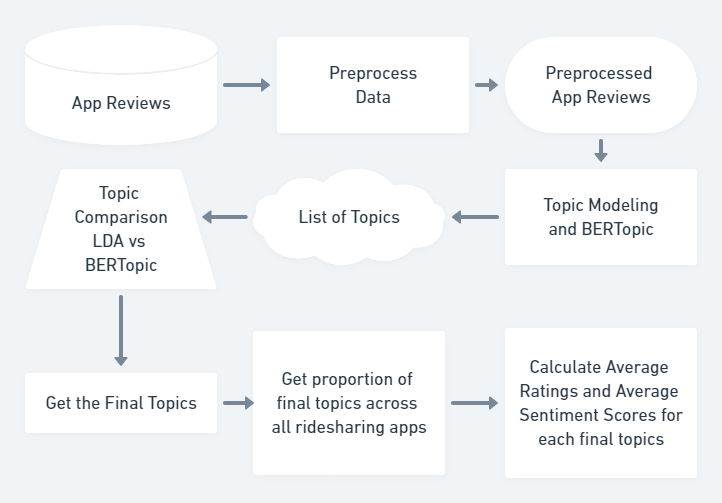
\includegraphics[width=\textwidth]{figures/image2.png}
\caption{Overview of the study setup}
\label{fig:overview_of_study_setup}
\end{center}
\end{figure}


\subsection{Data Collection Process}
In the first step, we collect app reviews from Google Play Store and Apple App Store. For Google Play Store, we used google-play-scraper \footnote{\url{https://github.com/JoMingyu/google-play-scraper}} developed by JoMingyu. For Apple App Store, we used app-store-scraper \footnote{\url{https://github.com/cowboy-bebug/app-store-scraper}} developed by \textit{cowboy-bebug}. Both libraries provide APIs in Python for app store data crawling. We stored the mining result in csv files. A reproducible jupyter notebook for mining the app review is available at this link\footnote{\url{https://github.com/enliktjioe/master-thesis-2021/tree/main/review_mining}}. 

Table \ref{tab:total_reviews_rating} shows the total number of app reviews and average ratings from each ridesharing app in both app stores and combines both numbers for general information for each app. 

\begin{table}[!h]
\caption{Total Reviews and Average Ratings from Google Play Store and Apple App Store}
\centering
\begin{tabular}{p{0.5cm}lp{1.5cm}lp{2cm}lp{2cm}lp{2cm}lp{2cm}lp{2cm}l}
\hline
\textbf{No} & \textbf{App Name} & \textbf{OS} & \begin{tabular}[c]{@{}l@{}}\textbf{Total}\\\textbf{Reviews}\end{tabular} & \begin{tabular}[c]{@{}l@{}}\textbf{Average}\\\textbf{Ratings}\end{tabular} & \begin{tabular}[c]{@{}l@{}}\textbf{TotalReviews}\\\textbf{Combined}\end{tabular} &
\begin{tabular}[c]{@{}l@{}}\textbf{AverageRatings}\\\textbf{Combined}\end{tabular}\\
\hline
1           & Bolt              & Android     & 51907                                                                    & 3.96                                                                       & 55061                                                                             & 3.91                               \\
           &                   & iOS         & 3154                                                                     & 3.02                                                                       &                                                                                   &                                    \\
2           & Uber              & Android     & 10000                                                                    & 3.3                                                                        & 20342                                                                             & 3.13                               \\
           &                   & iOS         & 10342                                                                    & 2.96                                                                       &                                                                                   &                                    \\
3           & BlaBlaCar         & Android     & 19452                                                                    & 4.3                                                                        & 44480                                                                             & 4.21                               \\
           &                   & iOS         & 23308                                                                    & 4.13                                                                       &                                                                                   &                                    \\
4           & Cabify            & Android     & 3261                                                                     & 2.6                                                                        & 10645                                                                             & 3.7                                \\
           &                   & iOS         & 7384                                                                     & 4.19                                                                       &                                                                                   &                                    \\
5           & Via               & Android     & 1873                                                                     & 3.6                                                                        & 4265                                                                              & 3.63                               \\
          &                   & iOS         & 2392                                                                     & 3.65                                                                       &                                                                                   &                                    \\
6           & Getaround         & Android     & 731                                                                      & 3.46                                                                       & 3219                                                                              & 3.3                                \\
            &                   & iOS         & 2488                                                                     & 3.25                                                                       &                                                                                   &                                    \\
7           & Ola Cabs          & Android     & 10000                                                                    & 1.54                                                                       & 10922                                                                             & 1.9                                \\
            &                   & iOS         & 922                                                                      & 2.19                                                                       &                                                                                   &                                    \\
8           & Taxi.eu           & Android     & 211                                                                      & 2.8                                                                        & 775                                                                               & 3.32                               \\
            &                   & iOS         & 564                                                                      & 3.52                                                                       &                                                                                   &                                    \\
9           & Free Now          & Android     & 11078                                                                    & 3.24                                                                       & 25428                                                                             & 3.52                               \\
            &                   & iOS         & 14350                                                                    & 3.73                                                                       &                                                                                   &                                    \\
10          & Yandex Go         & Android     & 7053                                                                     & 3.26                                                                       & 7224                                                                              & 3.25                               \\
\hline
\label{tab:total_reviews_rating}
\end{tabular}
\end{table}

\subsection{NLP Preprocessing}
Data preprocessing is needed to get a better quality of the dataset. To preprocess data means to transform it into a well-format dataset that we can use more effectively in a data science project.   \cite{text_preprocessing_nlp}. There are different types of text preprocessing techniques, including
\begin{enumerate}
  \item Lowercasing, mapping all words into the same lowercase form
  \item Stemming, transforming words into their root form, for example, ‘playing’ becomes ‘play’. Examples are listed in Figure \ref{fig:stemming}
  \item Lemmatization, similar to stimming, maps a word into its root form, but in a more proper way. Examples are listed in Figure \ref{fig:lemmatization}
  \item Stopword Removal, removing commonly used words in a language such as “a”, “the”, “is”, “are”, and so on.
\end{enumerate}


\begin{figure}[!h]
    \centering
    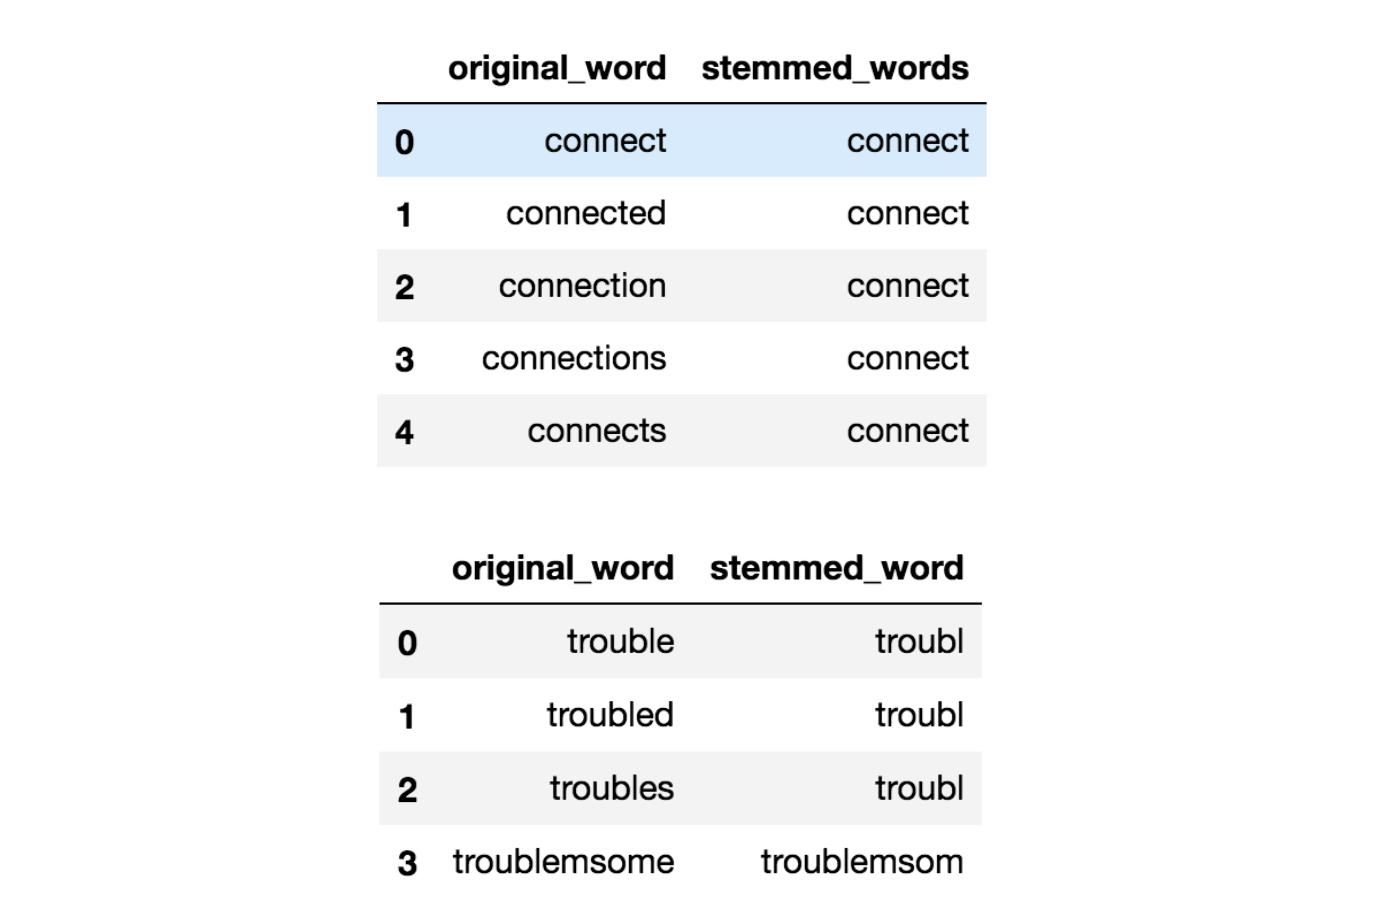
\includegraphics[width=0.5\textwidth]{figures/stemming.png}
    \caption{Example of Stemming}
    \label{fig:stemming}
\end{figure}

\begin{figure}[!h]
    \centering
    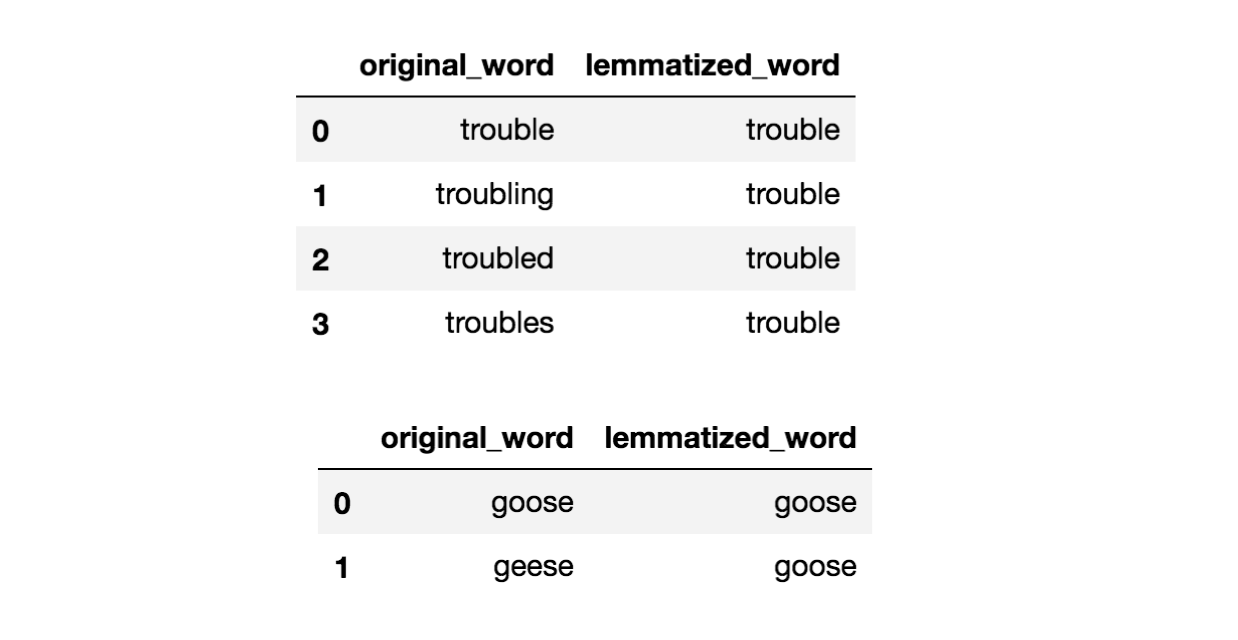
\includegraphics[width=0.5\textwidth]{figures/lemmatize.png}
    \caption{Example of Lemmatization}
    \label{fig:lemmatization}
\end{figure}



The study of Jiahao Weng \cite{text_preprocessing_nlp_2} tried to compare the result of text analysis with and without preprocessing steps. The authors stated how preprocessing could improve the accuracy of sentiment analysis by clearing the context of the analyzed sentence.

Before the first preprocessing steps (P1), we already did the basics of NLP preprocessing steps. These include lowercasing text, lemmatization, and stopword removal. After that, we started the planned preprocessing steps, including removing non-English reviews, filtering out inconsistent and uninformative reviews, correcting typos, and building a text corpus. Table \ref{tab:preprocessing_result} shows the total number of app reviews before and after each preprocessing step for every app. P1 is the first preprocessing step where we removed non-English app reviews. P2 is the second step where we removed inconsistent app reviews (star rating and sentiment are not matched). P3 is the third step where we remove uninformative reviews, which are usually short reviews that only include praise or dispraise (for example: “I love it,” “I hate this app”) according to Guzman et al. \cite{fine_grained}. In the following, we explain all these preprocessing steps in more detail.

\begin{table}[!h]
\caption{List of the Top 10 Ridesharing Apps, Followed by the Initial Number of User-Reviews, and Number of Consistent and Informative User-Reviews}
\centering
\hline 
\begin{tabular}{llllll}
\textbf{No} & \textbf{App Name} & \textbf{\#Reviews} & \begin{tabular}[c]{@{}l@{}}\textbf{(P1) English}\\\textbf{Reviews}\end{tabular} & \begin{tabular}[c]{@{}l@{}}\textbf{(P2) Consistent}\\\textbf{Reviews}\end{tabular} & \begin{tabular}[c]{@{}l@{}}\textbf{(P3) Informative}\\\textbf{Reviews}\end{tabular} \\
\hline
1              & Bolt             & 55061                    & 40365                         & 17930                            & 10785                              \\
2              & Uber             & 20342                    & 19833                         & 8285                             & 6763                               \\
3              & BlaBlaCar        & 44480                    & 16212                         & 8822                             & 3156                               \\
4              & Cabify           & 10645                    & 1899                          & 763                              & 551                                \\
5              & Via              & 4265                     & 3962                          & 1863                             & 1417                               \\
6              & Getaround        & 3219                     & 894                           & 365                              & 249                                \\
7              & Ola Cabs         & 10922                    & 10875                         & 3766                             & 3573                               \\
8              & Taxi.eu          & 775                      & 220                           & 72                               & 43                                 \\
9              & Free Now         & 25428                    & 10939                         & 4285                             & 2728                               \\
10             & Yandex Go        & 7224                     & 2888                          & 1261                             & 622                                \\
\hline
\textbf{Total} &                  & \textbf{\textit{182361}} & \textbf{\textit{108084}}      & \textbf{\textit{47412}}          & \textbf{\textit{29813}}           \\
\hline
\end{tabular}
\label{tab:preprocessing_result}
\end{table}
\subsubsection{Remove Non-English Reviews}
We found out that some app reviews we have collected contain non-English reviews. Most of the non-English reviews come from Apple App Store, as our data scraper for Apple App Store does not have a language filter parameter. We’re using the Python library name \textit{langdetect}\cite{langdetect} to remove around 70,000+ non-English app reviews. The languages in the non-English reviews are from European countries which not use English as the main language, such as Russia, Germany, and France.

The \textit{langdetect} library has a scoring system for every app review text, including the language code (two letters) and its probability score. The example of \textit{langdetect} library can be seen in Figure \ref{fig:langdetect_1}. In Figure \ref{fig:langdetect_2} when the app review is too short, it might give multiple language probability.

\begin{figure}[!h]
\begin{lstlisting}
detect_langs("Shared my promo code with my friend and didn’t get any discount. No live chat no way to text them")

[en:0.9999972783798426]

detect_langs("pourquoi ne pas afficher toutes les voitures disponibles autour du point de prise en charge ? faire des promos c’est bien mais si pas de voitures disponibles....des erreurs 7002 fréquentes, des indications de temps d’arrivée fantaisistes. Une fois le chauffeur sélectionné on s’aperçoit souvent qu’il finit une course et ça prend du temps ce qui fait que le compteur d’arrivée reste figé sur un temps d’attente « acceptable » pour bloquer l’usager mais qui peut facilement être le double de celui indiqué....")

[fr:0.9999982827184632]
\end{lstlisting}
\caption{Examples of \textit{langdetect} library}
\label{fig:langdetect_1}
\end{figure}

\begin{figure}[!h]
\begin{lstlisting}
detect_langs("Very fast and affordable")
[en:0.5714280394408676, da:0.42857192445741144]

detect_langs("Best app ever")
[no:0.7142813554856114,fr:0.1428580578700273, en:0.14285644644057932]

\end{lstlisting}
\caption{Examples of Multiple Languages Probability}
\label{fig:langdetect_2}
\end{figure}

% \begin{figure}
% \begin{lstlisting}
% Great experience with the drivers and very reasonably priced
% (True,'en:0.9999974406709471',0.9999974406709471)

% Less stressful Less expensive and Very confortable
% (True,'en:0.7142831849235615,fr:0.2857157947567049',0.7142831849235615)

% Przesympatyczny kierowca polecam ��
% (False, None, 0)

% Kezd ugyanolyan proli vacak lenni, mint a sima taxi. Most legutoljara a sofor 30 Ft-al tobbet utott bele az alkalmazasba, mint amit a taxiora mutatott. Pofatlan suttyo.
% (False, None, 0)
% \end{lstlisting}
% \caption{Examples of English/Non-English Review}
% \label{fig:langdetect_3}
% \end{figure}


To decide if it is English or non-English, we made a Python function to get an English ‘en’ probability score. If ‘en’ scores exceed 0.1, it will be categorized as English text. If ‘en’ score is below or equal to 0.1 or does not contain ‘en’ score, it will be categorized as non-English text. Here are the example results from the function,



\subsubsection{Remove Inconsistent Reviews}
Inconsistent reviews happen when users give negative reviews but give high star ratings instead. Similarly, users give positive reviews but give low star ratings instead. For example, the review text is “Horrible app, not user friendly,” but it was associated with five stars. To detect inconsistent reviews, we are using a comparison between star ratings with their sentiment score. We calculated the sentiment score using SentiStrength Python library \cite{sentistrength}, the wrapper for its original Java library.

SentiStrength gives scores to app reviews with a value ranging from -5 (most negative) to +5 (most positive). Sentiments with scores -5, -4, -3, and -2 are considered as negative sentiments, while scores -1, 0, and +1 as neutral sentiments, and +2, +3, +4, +5 are positive sentiments. For star rating, the possible values are between 1 and 5. Negative ratings are 1 and 2, neutral ratings are 3, and positive ratings are 4 and 5. Figure \ref{fig:example_of_consistent} shows the example of consistent app reviews. Figure \ref{fig:example_of_inconsistent} shows the example of inconsistent app reviews.

We kept only the consistent review in order to minimize the misinformation that can happen in our analysis. For example, an app review with a sentiment score of +4 and a rating of 5 will be considered a consistent review. Meanwhile, an app review with a sentiment score of +4 and a rating of -1 will be considered an inconsistent review. Table 6 shows the mapping of positive, neutral, and negative scores for both sentiment and rating.

\begin{figure}[!h]
\begin{center}
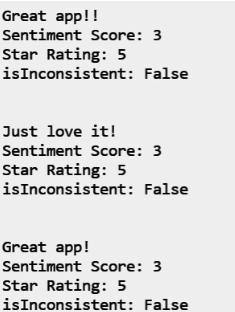
\includegraphics[width=0.2\textwidth]{figures/example_consistent_review.png}
\caption{Example of Consistent App Reviews}
\label{fig:example_of_consistent}
\end{center}
\end{figure}

\begin{figure}[!h]
\begin{center}
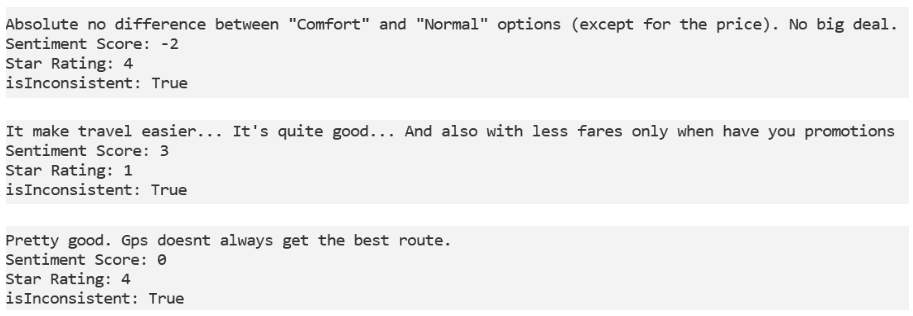
\includegraphics[width=1\textwidth]{figures/example_inconsistent_review.png}
\caption{Example of Inconsistent App Reviews}
\label{fig:example_of_inconsistent}
\end{center}
\end{figure}


\begin{table}[!h]
\centering
\caption{Detail of Sentiment and Rating Scoring System}
\begin{tabular}{| l | l | l |}
	\hline
	\bf{No} & \bf{Category} & \bf{Score(s)} \\
	\hline
	1 & Positive Sentiment & [+2, +3, +4, +5] \\
	\hline
	2 & Positive Rating & [4, 5] \\
	\hline
	3 & Neutral Sentiment & [-1, 0, +1] \\
	\hline
	4 & Neutral Rating & [3] \\
	\hline
	5 & Negative Sentiment & [-5, -4, -3, -2] \\
	\hline
	6 & Negative Rating & [1, 2] \\
	\hline
\end{tabular}
\label{tab:statements}
\end{table}


\newpage
\subsubsection{Remove Uninformative Reviews}
Some uninformative app reviews do not give app developers any beneficial information. We used the AR-Miner framework introduced by Chen et al.\cite{arminer}. As AR-Miner source code was not available publicly, we implemented the logic using the SVM (Support Vector Machine) classifier. Several examples of uninformative app reviews that we have found in our dataset:

\begin{itemize}
\itemsep0em
\item good and reasonable prices
\item amazing simple and suitable
\item a very good service provider
\item great prices great people
\item nice and easy to operate
\item it very easy and nice
\end{itemize}

Most uninformative reviews are short app reviews without significant information to analyze.

\subsubsection{Building Corpus}
The final step before running statistical analysis like topic modeling \cite{text_corpus} is to create a text corpus. Before building the text corpus, we normalize the app reviews, including removing the stop words, removing the punctuation, and lemmatizing the words. We used Gensim corpora library \cite{gensim} to create the text corpus and convert it into \textit{tf\_idf}\footnote{\url{https://radimrehurek.com/gensim/models/tfidfmodel.html}} format, short for \textbf{term frequency–inverse document frequency}. It is a numerical statistic that is intended to reflect how important a word is to a document in a collection or corpus \cite{rajaraman_ullman_2011}. We saved the corpus file into a binary file for Python named \textit{pickle}\footnote{\url{https://docs.python.org/3/library/pickle.html/}}. Figure \ref{fig:img_corpus} shows the example in Gensim to create \textit{tf\_idf} corpus using Jupyter Notebook. This binary file of \textit{tf\_idf} corpus will be used for Gensim's text classification and clustering framework.


\begin{figure}[!h]
\begin{center}
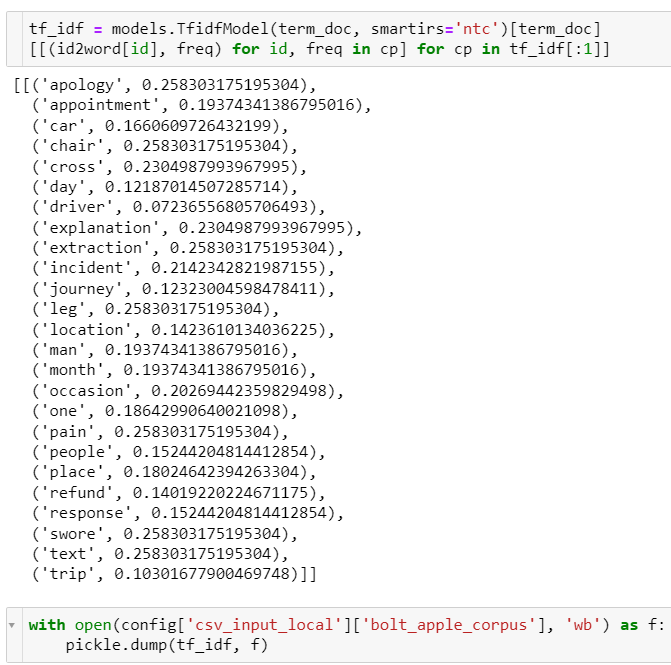
\includegraphics[width=0.7\textwidth]{figures/image19.png}
\caption{Using Gensim Corpora library to make Corpus file}
\label{fig:img_corpus}
\end{center}
\end{figure}

\newpage
\section{Implementation}
Topic modeling is one of the unsupervised machine learning techniques that is useful to discover the abstract “topic” from a collection of text documents. One of the most common algorithms for fitting a topic modeling is Latent Dirichlet Allocation (LDA). It will map each document in the text corpus to a set of topics that represent a group of words in the document. An example of a topic can be the set of words {location, map, app, address, area} which describes users’ experiences when checking location using the ridesharing app. In LDA, every document is a combination of topics, and every topic is a combination of words \cite{text_mining_R}. Figure \ref{fig:img_lda_topic_modeling_example} shows the example of topic modeling result using the LDA technique.


\begin{figure}[h]
\begin{center}
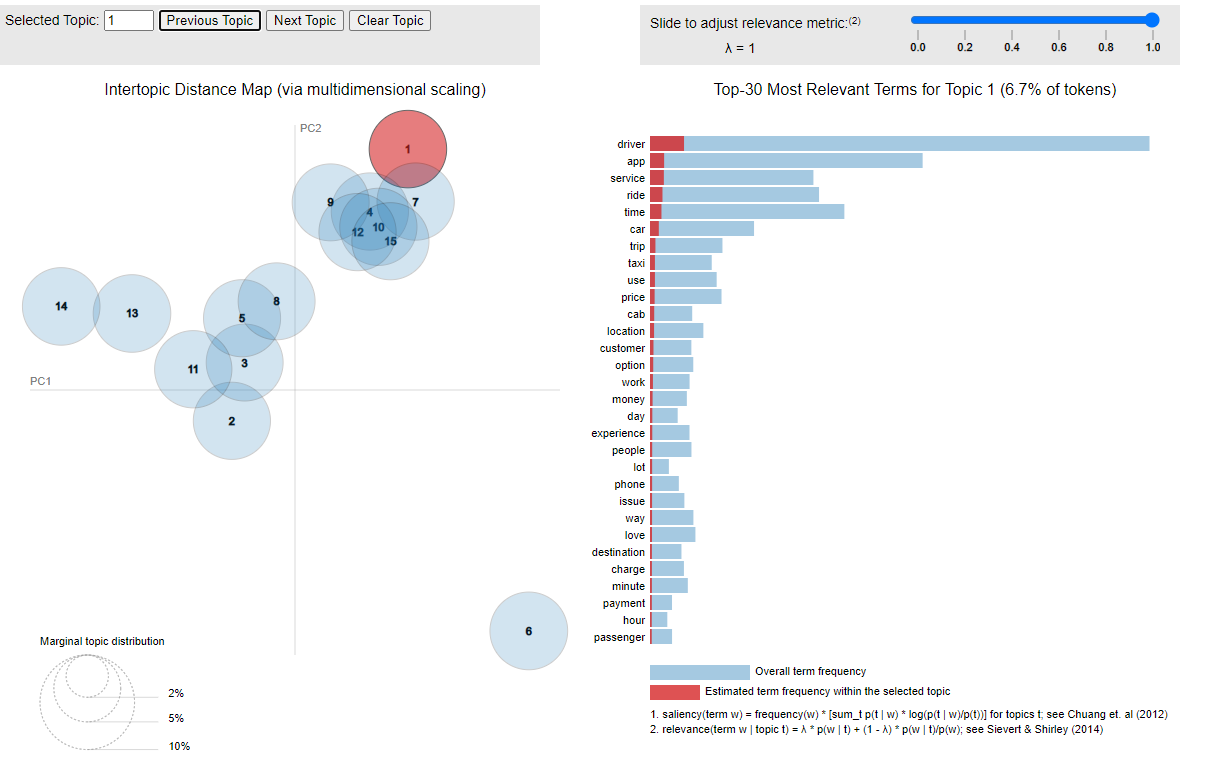
\includegraphics[width=0.7\textwidth]{figures/image9.png}
\caption{Example of Topics created by LDA}
\label{fig:img_lda_topic_modeling_example}
\end{center}
\end{figure}

Each app review contains some contexts that will be useful if we can understand them. LDA is one of the most popular topic modeling techniques. We use Gensim as one of the most widely-used Python libraries for implementing LDA Topic Modeling. Other than LDA, we are also using Pre-Trained Model BERT to implement topic modeling, utilizing an open-source library named BERTopic \cite{bertopic}.

To find the optimal number of topics, we compute coherence scores using different topics ranging from 2 to 40, as shown in Figure \ref{fig:img_coherence_score}. We chose 20 as the number of optimal topics as this number gave the highest value before the coherence score flattened out.
\newline

\begin{figure}
\begin{center}
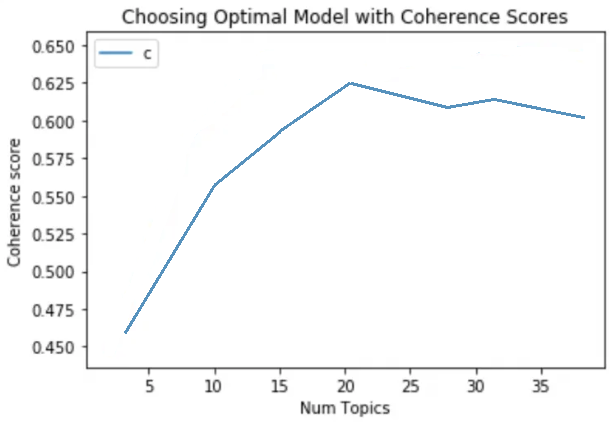
\includegraphics[width=0.7\textwidth]{figures/image17.png}
\caption{Coherence Score per Number of Topics}
\label{fig:img_coherence_score}
\end{center}
\end{figure}


\begin{table}[!h]
\caption{Coherence Score for Different Topic Modeling Techniques using 20 Topics}
\centering
\begin{tabular}{llllll}
\hline
\begin{tabular}[c]{@{}l@{}}\\\textbf{Dataset}\end{tabular} & \begin{tabular}[c]{@{}l@{}}\textbf{\#Reviews~}\\\textbf{(BEFORE)}\end{tabular} & \begin{tabular}[c]{@{}l@{}}\textbf{\#Reviews}\\\textbf{(AFTER)}\end{tabular} & \textbf{LDA}\textbf{ Standard}    & \textbf{LDA}\textbf{ Mallet} & \textbf{BERTopic}  \\
\hline
Bolt P1 (\\Remove \\Non-English \\Reviews)                       & 55061                                                                          & 40365                                                                        & 0.3156                   & 0.4268              & \textbf{0.4410}    \\
\hline
Bolt P2 (P1 + \\Remove \\Inconsistent \\Reviews)                 & 40365                                                                          & 17930                                                                        & 0.4139                   & \textbf{0.4874}     & 0.4152             \\
\hline
Bolt P3 (P2 + \\Remove \\Uninformative \\Reviews)                & 17930                                                                          & 10785                                                                        & 0.4051                   & \textbf{0.4905}     & 0.4518  \\
\hline
\end{tabular}
\label{tab:coherence_score}
\end{table}


We realized that the data preprocessing step has filtered out more than 50\% of the total app reviews by comparing the coherence score from three different datasets and three different topic modeling approaches. We used Bolt app reviews because it has the highest number of app reviews compared to the other nine ridesharing apps, and we thought it was enough to get a coherence score comparison. Table \ref{tab:coherence_score} shows the total number of app reviews from Bolt app using three different datasets and its coherence score for three different topic modeling approaches. Based on coherence score comparison, we selected two out of three methods for topic modeling comparison, LDA Mallet and BERTopic, as both perform better compared to the LDA Standard model. In the following, we explain the topic result from both LDA Mallet and BERTopic.

\subsection{LDA Mallet}
Mallet (MAchine Learning for LanguagE Toolkit) \cite{mallet} is a java-based open-source toolkit written by Andrew McCallum and used for many machine learning applications to text, including Topic Modeling. Gensim is a Python library that provides a wrapper for LDA. To use LDA Mallet in Gensim, we can call the module with syntax gensim.models.wrappers.LdaMallet. This module contains Gibbs sampling from Mallet that allows LDA model to get the topic result from the unseen documents. Table \ref{tab:lda_mallet_tm} shows all 20 topics based on the top 10 keywords extracted using LDA Mallet technique. LDA technique only puts the topic as a number, so we need to label it manually. There are several topics with the same name because it has very similar keywords, and we decide to give the same one.


\begin{table}[!h]
\caption{LDA Mallet Topic Modeling using Bolt P3 dataset}
\label{tab:lda_mallet_tm}
\centering
\hline
\begin{tabular}{llll}
\textbf{No}                            & \begin{tabular}[c]{@{}l@{}}\textbf{Topic}\\\textbf{Name}\end{tabular}                                                              & \textbf{Keywords}                                                                                                                                         & \textbf{Counts}  \\
\hline
\textcolor[rgb]{0.067,0.067,0.067}{1}  & \textcolor[rgb]{0.067,0.067,0.067}{Price}                                                                                          & \begin{tabular}[c]{@{}l@{}}price, destination, experience, friendly\_driver, change, \\easy\_use, competitor, good\_price, comfort, increase\end{tabular} & 2234             \\
2                                      & \begin{tabular}[c]{@{}l@{}}Praising \\Features\end{tabular}                                                                        & \begin{tabular}[c]{@{}l@{}}service, love, life, fast\_efficient, download, \\rude, affordable\_price, mind, availability, really\_good\end{tabular}       & 764              \\
\textcolor[rgb]{0.067,0.067,0.067}{3}  & \textcolor[rgb]{0.067,0.067,0.067}{Time}                                                                                           & \begin{tabular}[c]{@{}l@{}}time, taxi, drivers\_alway, point,pricing, \\pickup, travel, driving, drop, order\end{tabular}                                 & 762              \\
\textcolor[rgb]{0.067,0.067,0.067}{4}  & \textcolor[rgb]{0.067,0.067,0.067}{Location}                                                                                       & \begin{tabular}[c]{@{}l@{}}location, map, app, address, area, \\order, pick, feature, improvement, street\end{tabular}                                    & 628              \\
\textcolor[rgb]{0.067,0.067,0.067}{5}  & \begin{tabular}[c]{@{}l@{}}\textcolor[rgb]{0.067,0.067,0.067}{Driver }\\\textcolor[rgb]{0.067,0.067,0.067}{Service}\end{tabular}   & \begin{tabular}[c]{@{}l@{}}driver, app, phone, lot, man, move,\\~booking, cancel\_trip, drive, instance\end{tabular}                                      & 577              \\
\textcolor[rgb]{0.067,0.067,0.067}{6}  & \begin{tabular}[c]{@{}l@{}}\textcolor[rgb]{0.067,0.067,0.067}{Driver }\\\textcolor[rgb]{0.067,0.067,0.067}{Service}\end{tabular}   & \begin{tabular}[c]{@{}l@{}}driver, experience, client, end, rating, cancel, \\condition, music, professional, conversation\end{tabular}                   & 509              \\
\textcolor[rgb]{0.067,0.067,0.067}{7}  & \begin{tabular}[c]{@{}l@{}}\textcolor[rgb]{0.067,0.067,0.067}{User }\\\textcolor[rgb]{0.067,0.067,0.067}{Experience}\end{tabular}  & \begin{tabular}[c]{@{}l@{}}work, issue, thing, traffic, friend, \\drive, scam, user, transport, yesterday\end{tabular}                                    & 503              \\
\textcolor[rgb]{0.067,0.067,0.067}{8}  & \textcolor[rgb]{0.067,0.067,0.067}{Driver}                                                                                         & \begin{tabular}[c]{@{}l@{}}driver, passenger, vehicle, case, city, scooter, \\transportation, arrival, item, promotion\end{tabular}                       & 492              \\
\textcolor[rgb]{0.067,0.067,0.067}{9}  & \begin{tabular}[c]{@{}l@{}}\textcolor[rgb]{0.067,0.067,0.067}{Customer }\\\textcolor[rgb]{0.067,0.067,0.067}{Support}\end{tabular} & \begin{tabular}[c]{@{}l@{}}service, charge, email, cab, month, \\hour, reply, good, year, person\end{tabular}                                             & 482              \\
\textcolor[rgb]{0.067,0.067,0.067}{10} & \textcolor[rgb]{0.067,0.067,0.067}{Payment}                                                                                        & \begin{tabular}[c]{@{}l@{}}card, money, problem, pay, account, application, \\detail, error, card\_payment, report\end{tabular}                           & 450              \\
\textcolor[rgb]{0.067,0.067,0.067}{11} & \begin{tabular}[c]{@{}l@{}}\textcolor[rgb]{0.067,0.067,0.067}{Ride }\\\textcolor[rgb]{0.067,0.067,0.067}{Experience}\end{tabular}  & \begin{tabular}[c]{@{}l@{}}customer, company, route, driver, journey, \\reason, refund, safety, review, screen\end{tabular}                               & 418              \\
\textcolor[rgb]{0.067,0.067,0.067}{12} & \begin{tabular}[c]{@{}l@{}}\textcolor[rgb]{0.067,0.067,0.067}{User }\\\textcolor[rgb]{0.067,0.067,0.067}{Experience}\end{tabular}  & \begin{tabular}[c]{@{}l@{}}trip, option, fare, rider, business, \\star, complain, stop, charge, travel\end{tabular}                                       & 407             \\
\hline
\end{tabular}
\end{table}

\begin{table}[!h]
\centering
\begin{tabular}{llll}
\hline
\textcolor[rgb]{0.067,0.067,0.067}{13} & \begin{tabular}[c]{@{}l@{}}\textcolor[rgb]{0.067,0.067,0.067}{Ride }\\\textcolor[rgb]{0.067,0.067,0.067}{Experience}\end{tabular}  & \begin{tabular}[c]{@{}l@{}}car, driver, system, team, quality, \\book, bit, woman, world, attitude\end{tabular}                                           & 399              \\
\textcolor[rgb]{0.067,0.067,0.067}{14} & \begin{tabular}[c]{@{}l@{}}\textcolor[rgb]{0.067,0.067,0.067}{Ride }\\\textcolor[rgb]{0.067,0.067,0.067}{Experience}\end{tabular}  & \begin{tabular}[c]{@{}l@{}}ride, cash, show, notification, fix, enjoy, \\amazing\_service, ad, period, purpose\end{tabular}                               & 396              \\
\textcolor[rgb]{0.067,0.067,0.067}{15} & \begin{tabular}[c]{@{}l@{}}\textcolor[rgb]{0.067,0.067,0.067}{Driver }\\\textcolor[rgb]{0.067,0.067,0.067}{Service}\end{tabular}   & \begin{tabular}[c]{@{}l@{}}driver, call, place, road, pick\_location, \\today, datum, kind, occasion, side\end{tabular}                                   & 338              \\       
\textcolor[rgb]{0.067,0.067,0.067}{16} & \begin{tabular}[c]{@{}l@{}}\textcolor[rgb]{0.067,0.067,0.067}{Customer }\\\textcolor[rgb]{0.067,0.067,0.067}{Support}\end{tabular} & \begin{tabular}[c]{@{}l@{}}guy, people, response, number, payment, \\code, complaint, message, lot, situation\end{tabular}                                & 321              \\
\textcolor[rgb]{0.067,0.067,0.067}{17} & \begin{tabular}[c]{@{}l@{}}\textcolor[rgb]{0.067,0.067,0.067}{Driver }\\\textcolor[rgb]{0.067,0.067,0.067}{Service}\end{tabular}   & \begin{tabular}[c]{@{}l@{}}driver, day, support, promo, amount, promotion, \\week, recommend, customer\_service, job\end{tabular}                         & 320              \\
\textcolor[rgb]{0.067,0.067,0.067}{18} & \begin{tabular}[c]{@{}l@{}}\textcolor[rgb]{0.067,0.067,0.067}{Feature }\\\textcolor[rgb]{0.067,0.067,0.067}{Request}\end{tabular}  & \begin{tabular}[c]{@{}l@{}}app, request, update, estimate, \\cost, fee, min, today, rubbish, arrival\end{tabular}                                         & 300              \\
\textcolor[rgb]{0.067,0.067,0.067}{19} & \textcolor[rgb]{0.067,0.067,0.067}{Time}                                                                                           & \begin{tabular}[c]{@{}l@{}}time, driver, minute, direction, distance, \\estimation, airport, load, great\_experience, talk\end{tabular}                   & 288              \\
\textcolor[rgb]{0.067,0.067,0.067}{20} & \textcolor[rgb]{0.067,0.067,0.067}{Promotion}                                                                                      & \begin{tabular}[c]{@{}l@{}}app, discount, rate, network, share, info, \\a lot, experience, convenience, comment\end{tabular}                              & 197   \\     
\hline     
\end{tabular}
\end{table}

\newpage
\subsection{BERTopic}
Bidirectional Encoder Representations from Transformers (BERT) is one of the best NLP pre-training models developed by Google and released as an open source project in 2018. It was pre-trained using massive amounts of text data from English Wikipedia. In its research stages, BERT achieved revolutionary results in 11 natural language understanding tasks, including sentiment analysis, sentence classification, semantic role labeling, and disambiguation of words with multiple meanings. It effectively addresses ambiguity, which is the greatest challenge in natural language understanding. BERT gives the capability to parse the human language with a relatively human-like common sense.

Meanwhile, BERTopic \cite{bertopic} is a topic modeling tool developed by Marteen Grootendorst in 2020 that utilizes Transformers to create dense clusters allowing for easily interpretable topics while keeping important words in the topic description. Figure \ref{fig:img_bertopic_main_components} shows the BERTopic components based on its official documentation. Table \ref{tab:bertopic_result} shows 20 topics extracted using BERTopic, including its top 4 keywords. Similar to the previous technique, we needed to label these topics manually and got several topics with the same name.

\begin{figure}[!h]
\begin{center}
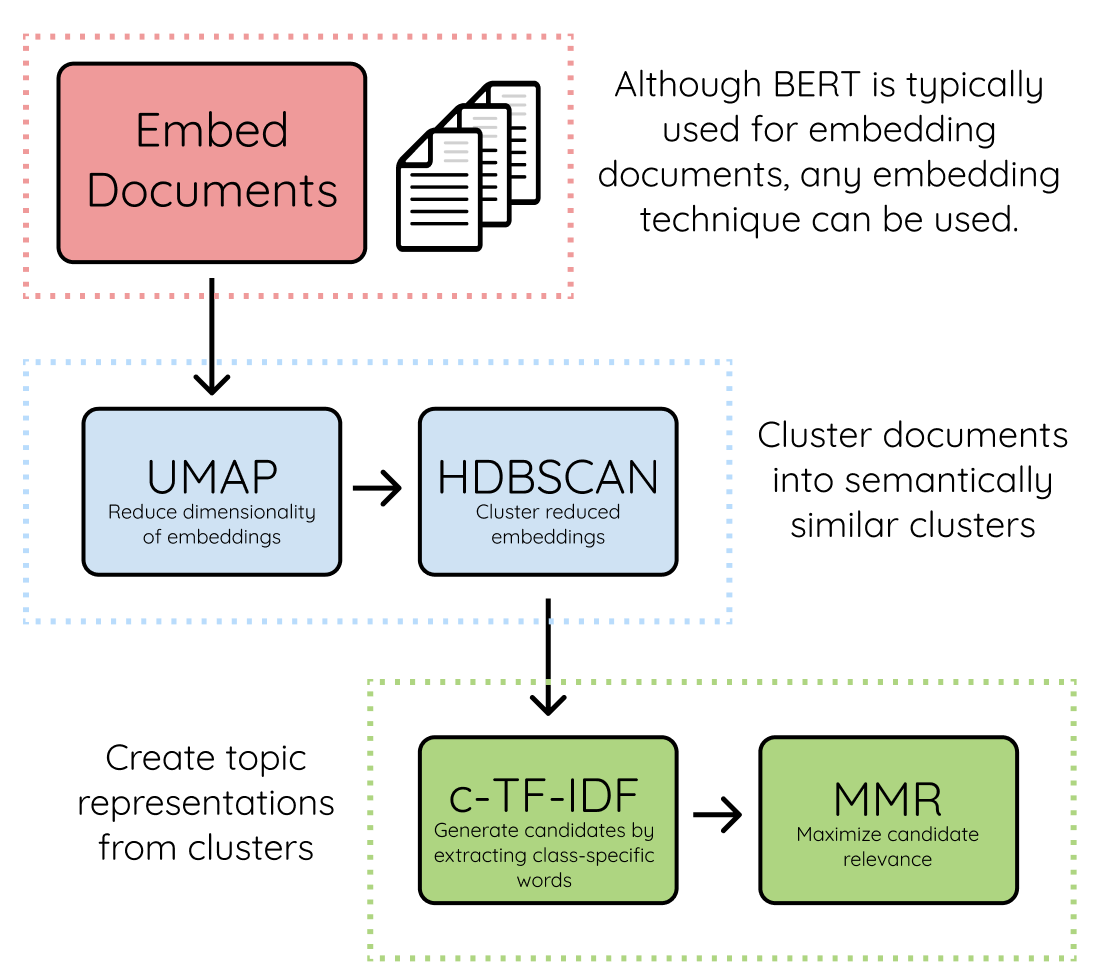
\includegraphics[width=0.525\textwidth]{figures/image24.png}
\caption{BERTopic Main Components}
\label{fig:img_bertopic_main_components}
\end{center}
\end{figure}

\begin{table}[!h]
\caption{BERTopic Topic Modeling using BOLT P3 Dataset}
\centering
\begin{tabular}{llll}
\hline
\textbf{No} & \textbf{Topic}    & \textbf{Keywords}                          & \textbf{Count}  \\
\hline
N/A         & (OUTLIER)         & -1\_app\_my\_driver\_on                    & 3371            \\
1           & Driver Service    & 0\_drivers\_friendly\_good\_nice           & 1920            \\
2           & Driver Service    & 1\_app\_drivers\_good\_friendly            & 467             \\
3           & Pricing           & 2\_prices\_discounts\_price\_good          & 455             \\
4           & Praising Features & 3\_service\_reliable\_great\_excellent     & 429             \\
5           & Ride Experience   & 4\_ride\_rides\_enjoyed\_enjoy             & 428             \\
6           & Driver Service    & 5\_bolt\_was\_driver\_but                  & 362             \\
7           & Praising Features & 6\_efficient\_reliable\_app\_good          & 360             \\
8           & Praising Features & 7\_experience\_keep\_enjoy\_love           & 304             \\
9           & Praising Features & 8\_bolt\_experience\_good\_awesome         & 298             \\
10          & Pricing           & 9\_affordable\_good\_efficient\_nice       & 291             \\
11          & Location          & 10\_location\_app\_pick\_my                & 286             \\
12          & Ride Experience   & 11\_taxify\_taxi\_my\_this                 & 275             \\
13          & Driver Service    & 12\_driver\_he\_my\_code                   & 240             \\
14          & Praising Features & 13\_transport\_transportation\_trips\_easy & 231             \\
15          & Time              & 14\_minutes\_time\_waiting\_wait           & 190             \\
16          & Location          & 15\_gps\_map\_location\_maps               & 189             \\
17          & Praising Features & 16\_uber\_better\_cheaper\_more            & 182             \\
18          & Payment           & 17\_card\_payment\_account\_app            & 174             \\
19          & Driver Service    & 18\_rude\_drivers\_they\_worst             & 167             \\
20          & Promotion         & 19\_promo\_promos\_code\_promotions        & 166   \\
\hline
\end{tabular}
\label{tab:bertopic_result}
\end{table}

\clearpage
\newpage
\section{Findings and Analysis}
In this chapter, some findings and analysis were discussed to determine what is going well and what is the thing that can be improved for future improvement.

\subsection{Final Results}
Based on the LDA Mallet and BERTopic results above, we do the manual analysis to interpret the LDA model and select the final topics. We merge some topics with very similar meanings based on the keyword given by the model and the related app reviews. We follow these criteria before merging the topics:

\begin{itemize}
\item One topic consists of multiple keywords that we will use to compare with other keywords from different topics. If the keywords have similar meanings, we merge them into one topic.
\item If the keywords are not clear enough, we will look into the app review related to each topic. If the app reviews explain the same context, we merge them into the same group.
\end{itemize}

All final 13 topics are listed in Table \ref{tab:final_topics}, followed by the top five words and a brief description of each topic.

\begin{table}[!h]
\caption{The List of Identified Topics from App Reviews}
\centering
\begin{tabular}{llll}
\hline
\textcolor[rgb]{0.067,0.067,0.067}{\textbf{No}}  & \textcolor[rgb]{0.067,0.067,0.067}{\textbf{Topic Name}}                                                                             & \textcolor[rgb]{0.067,0.067,0.067}{\textbf{Top 5 Words}}                                                                                                               & \textcolor[rgb]{0.067,0.067,0.067}{\textbf{Brief Description}}                                                                                                                              \\
\hline
\textcolor[rgb]{0.067,0.067,0.067}{\textit{T1}}  & \begin{tabular}[c]{@{}l@{}}\textcolor[rgb]{0.067,0.067,0.067}{Reporting }\\\textcolor[rgb]{0.067,0.067,0.067}{Issues}\end{tabular}  & \begin{tabular}[c]{@{}l@{}}\textcolor[rgb]{0.067,0.067,0.067}{issue, scam, response, }\\\textcolor[rgb]{0.067,0.067,0.067}{problem, error}\end{tabular}                & \begin{tabular}[c]{@{}l@{}}\textcolor[rgb]{0.067,0.067,0.067}{Reporting issues about }\\\textcolor[rgb]{0.067,0.067,0.067}{the app features}\end{tabular}                                   \\
\textcolor[rgb]{0.067,0.067,0.067}{\textit{T2}}  & \begin{tabular}[c]{@{}l@{}}\textcolor[rgb]{0.067,0.067,0.067}{Customer }\\\textcolor[rgb]{0.067,0.067,0.067}{Support}\end{tabular}  & \begin{tabular}[c]{@{}l@{}}\textcolor[rgb]{0.067,0.067,0.067}{support, email, people, }\\\textcolor[rgb]{0.067,0.067,0.067}{response, call}\end{tabular}               & \begin{tabular}[c]{@{}l@{}}\textcolor[rgb]{0.067,0.067,0.067}{Customer’s complaint via }\\\textcolor[rgb]{0.067,0.067,0.067}{the customer support~}\end{tabular}                            \\
\textcolor[rgb]{0.067,0.067,0.067}{\textit{T3}}  & \begin{tabular}[c]{@{}l@{}}\textcolor[rgb]{0.067,0.067,0.067}{Driver }\\\textcolor[rgb]{0.067,0.067,0.067}{Service}\end{tabular}    & \begin{tabular}[c]{@{}l@{}}\textcolor[rgb]{0.067,0.067,0.067}{driver, problem, cancel, }\\\textcolor[rgb]{0.067,0.067,0.067}{rude, conversation}\end{tabular}          & \textcolor[rgb]{0.067,0.067,0.067}{Reviews related to driver's behavior}                                                                                                                    \\
\textcolor[rgb]{0.067,0.067,0.067}{\textit{T4}}  & \begin{tabular}[c]{@{}l@{}}\textcolor[rgb]{0.067,0.067,0.067}{Feature }\\\textcolor[rgb]{0.067,0.067,0.067}{Requests}\end{tabular}  & \begin{tabular}[c]{@{}l@{}}\textcolor[rgb]{0.067,0.067,0.067}{app, taxi, experience, }\\\textcolor[rgb]{0.067,0.067,0.067}{access, improvement}\end{tabular}           & \begin{tabular}[c]{@{}l@{}}\textcolor[rgb]{0.067,0.067,0.067}{Reviews related to additional }\\\textcolor[rgb]{0.067,0.067,0.067}{feature request}\end{tabular}                             \\
\textcolor[rgb]{0.067,0.067,0.067}{\textit{T5}}  & \textcolor[rgb]{0.067,0.067,0.067}{Location}                                                                                        & \begin{tabular}[c]{@{}l@{}}\textcolor[rgb]{0.067,0.067,0.067}{location, address, }\\\textcolor[rgb]{0.067,0.067,0.067}{direction, map, gps}\end{tabular}               & \begin{tabular}[c]{@{}l@{}}\textcolor[rgb]{0.067,0.067,0.067}{App experience when user choose }\\\textcolor[rgb]{0.067,0.067,0.067}{pickup and destination location}\end{tabular}           \\
\textcolor[rgb]{0.067,0.067,0.067}{\textit{T6}}  & \textcolor[rgb]{0.067,0.067,0.067}{Payment}                                                                                         & \begin{tabular}[c]{@{}l@{}}\textcolor[rgb]{0.067,0.067,0.067}{card, money, refund, }\\\textcolor[rgb]{0.067,0.067,0.067}{cash, change}\end{tabular}                    & \textcolor[rgb]{0.067,0.067,0.067}{Payment-related issues}                                                                                                                                  \\
\textcolor[rgb]{0.067,0.067,0.067}{\textit{T7}}  & \begin{tabular}[c]{@{}l@{}}\textcolor[rgb]{0.067,0.067,0.067}{Praising }\\\textcolor[rgb]{0.067,0.067,0.067}{Features}\end{tabular} & \begin{tabular}[c]{@{}l@{}}\textcolor[rgb]{0.067,0.067,0.067}{easy, convenience, safe, }\\\textcolor[rgb]{0.067,0.067,0.067}{fast\_affordable, efficient}\end{tabular} & \begin{tabular}[c]{@{}l@{}}\textcolor[rgb]{0.067,0.067,0.067}{Positive feedback given by user }\\\textcolor[rgb]{0.067,0.067,0.067}{about the overall experiences}\end{tabular}             \\
\textcolor[rgb]{0.067,0.067,0.067}{\textit{T8}}  & \textcolor[rgb]{0.067,0.067,0.067}{Pricing}                                                                                         & \begin{tabular}[c]{@{}l@{}}\textcolor[rgb]{0.067,0.067,0.067}{price, money, discount, }\\\textcolor[rgb]{0.067,0.067,0.067}{cheap, affordable}\end{tabular}            & \textcolor[rgb]{0.067,0.067,0.067}{Reviews related to app pricing}                                                                                                                          \\
\textcolor[rgb]{0.067,0.067,0.067}{\textit{T9}}  & \textcolor[rgb]{0.067,0.067,0.067}{Promotion}                                                                                       & \begin{tabular}[c]{@{}l@{}}\textcolor[rgb]{0.067,0.067,0.067}{promotion, request, }\\\textcolor[rgb]{0.067,0.067,0.067}{discount, code, service}\end{tabular}          & \textcolor[rgb]{0.067,0.067,0.067}{Reviews related to in-app promotion}                                                                                                                     \\
\textcolor[rgb]{0.067,0.067,0.067}{\textit{T10}} & \begin{tabular}[c]{@{}l@{}}\textcolor[rgb]{0.067,0.067,0.067}{Purpose }\\\textcolor[rgb]{0.067,0.067,0.067}{of Ride}\end{tabular}   & \begin{tabular}[c]{@{}l@{}}\textcolor[rgb]{0.067,0.067,0.067}{taxi, transport, work, }\\\textcolor[rgb]{0.067,0.067,0.067}{family, scooter}\end{tabular}               & \begin{tabular}[c]{@{}l@{}}\textcolor[rgb]{0.067,0.067,0.067}{The purpose of riding is for work, }\\\textcolor[rgb]{0.067,0.067,0.067}{visiting family, and using a scooter.}\end{tabular}  \\
\textcolor[rgb]{0.067,0.067,0.067}{\textit{T11}} & \begin{tabular}[c]{@{}l@{}}\textcolor[rgb]{0.067,0.067,0.067}{Ride }\\\textcolor[rgb]{0.067,0.067,0.067}{Experience}\end{tabular}   & \begin{tabular}[c]{@{}l@{}}\textcolor[rgb]{0.067,0.067,0.067}{ride, rate, enjoy, }\\\textcolor[rgb]{0.067,0.067,0.067}{easy\_use, passenger}\end{tabular}              & \begin{tabular}[c]{@{}l@{}}\textcolor[rgb]{0.067,0.067,0.067}{Reviews related to user’s }\\\textcolor[rgb]{0.067,0.067,0.067}{ride experience}\end{tabular}                                 \\
\textcolor[rgb]{0.067,0.067,0.067}{\textit{T12}} & \textcolor[rgb]{0.067,0.067,0.067}{Safety}                                                                                          & \begin{tabular}[c]{@{}l@{}}\textcolor[rgb]{0.067,0.067,0.067}{safe, night service, }\\\textcolor[rgb]{0.067,0.067,0.067}{journey, experience}\end{tabular}             & \begin{tabular}[c]{@{}l@{}}\textcolor[rgb]{0.067,0.067,0.067}{Reviews related to the safety of }\\\textcolor[rgb]{0.067,0.067,0.067}{ride experience}\end{tabular}                          \\
\textcolor[rgb]{0.067,0.067,0.067}{\textit{T13}} & \textcolor[rgb]{0.067,0.067,0.067}{Time}                                                                                            & \begin{tabular}[c]{@{}l@{}}\textcolor[rgb]{0.067,0.067,0.067}{time, minute, wait, }\\\textcolor[rgb]{0.067,0.067,0.067}{arrival, pickup}\end{tabular}                  & \begin{tabular}[c]{@{}l@{}}\textcolor[rgb]{0.067,0.067,0.067}{Reviews related to time spent for }\\\textcolor[rgb]{0.067,0.067,0.067}{pick up and arrival}\end{tabular} 
\end{tabular}
\hline
\label{tab:final_topics}
\end{table}

\clearpage
\newpage
\subsection{Proportion of Topics Across 10 Apps}
Several topics frequently appear in a specific app, while other topics appear infrequently. For example, in Getaround app, users mentioned more about customer support than promotion. It could be that Getaround app did not give much promotion compared to other ridesharing apps.

Table \ref{tab:proportion} shows the proportion of topics in each ridesharing app. We put bold text in the table cell to highlight the topic contributing at least ten percent of total reviews. Topic "praising features" frequently appeared in most apps except Ola Cabs. Getaround has the highest proportion of topic customer support compared to the other nine ridesharing app. Ridesharing app users are more likely to praise the app feature (praising features) more than report the app issue (reporting issues) or request a new feature (feature request). For more performance analysis of each topic, we used the average rating and average sentiment score as the metric in the following.


\begin{table}[!h]
\caption{Proportion of the Topics in Different Ridesharing Apps}
\centering
\begin{tabular}{llllllllllll}
\hline
\textbf{No} & \begin{tabular}[c]{@{}l@{}}\textbf{Topic}\\\textbf{Name}\end{tabular}
& \textbf{Bolt} & \textbf{Uber} & \begin{tabular}[c]{@{}l@{}}\textbf{Bla}\\\textbf{bla}\\\textbf{car}\end{tabular} & \begin{tabular}[c]{@{}l@{}}\textbf{Ca}\\\textbf{bify}\end{tabular} & \textbf{Via} & \begin{tabular}[c]{@{}l@{}}\textbf{Get}\\\textbf{aro}\\\textbf{und}\end{tabular} & \begin{tabular}[c]{@{}l@{}}\textbf{Ola}\\\textbf{Cabs}\end{tabular} & \begin{tabular}[c]{@{}l@{}}\textbf{Taxi}\\\textbf{.eu}\end{tabular} & \begin{tabular}[c]{@{}l@{}}\textbf{Free}\\\textbf{now}\end{tabular} & \begin{tabular}[c]{@{}l@{}}\textbf{Yan}\\\textbf{dex }\\\textbf{Go}\end{tabular}  \\
\hline
T1          & \begin{tabular}[c]{@{}l@{}}\textcolor[rgb]{0.067,0.067,0.067}{Reporting }\\\textcolor[rgb]{0.067,0.067,0.067}{Issues}\end{tabular}  & 4\%           & 4\%           & 3\%                                                                   & 4\%                                                                & 4\%          & 7\%                                                                   & 6\%                                                                 & 0\%                                                                 & 3\%                                                                 & 6\%                                                                               \\
T2          & \begin{tabular}[c]{@{}l@{}}\textcolor[rgb]{0.067,0.067,0.067}{Customer }\\\textcolor[rgb]{0.067,0.067,0.067}{Support}\end{tabular}  & 4\%           & 5\%           & 5\%                                                                   & 7\%                                                                & 5\%          & \textbf{25\%}}                                                           & 3\%                                                                 & 2\%                                                                 & 3\%                                                                 & 6\%                                                                               \\
T3          & \begin{tabular}[c]{@{}l@{}}\textcolor[rgb]{0.067,0.067,0.067}{Driver }\\\textcolor[rgb]{0.067,0.067,0.067}{Service}\end{tabular}    & \textbf{13\%}}          & \textbf{13\%}}         & \textbf{22\%}}                                                                  & \textbf{10\%}}                                                              & \textbf{12\%}}         & \textbf{15\%}}                                                                  & \textbf{12\%}}                                                                & 2\%                                                                 & 7\%                                                                 & \textbf{10\%}}                                                                             \\
T4          & \begin{tabular}[c]{@{}l@{}}\textcolor[rgb]{0.067,0.067,0.067}{Feature }\\\textcolor[rgb]{0.067,0.067,0.067}{Request}\end{tabular}   & 6\%           & 4\%           & 4\%                                                                   & 3\%                                                                & 5\%          & 4\%                                                                   & 3\%                                                                 & 9\%                                                                 & 5\%                                                                 & 5\%                                                                               \\
T5          & \textcolor[rgb]{0.067,0.067,0.067}{Location}                                                                                        & 4\%           & 4\%           & 1\%                                                                   & 3\%                                                                & 7\%          & 3\%                                                                   & 3\%                                                                 & 2\%                                                                 & 4\%                                                                 & 2\%                                                                               \\
T6          & \textcolor[rgb]{0.067,0.067,0.067}{Payment}                                                                                         & 6\%           & 6\%           & 4\%                                                                   & 8\%                                                                & 8\%          & 5\%                                                                   & 3\%                                                                 & 5\%                                                                 & 5\%                                                                 & 6\%                                                                               \\
T7          & \begin{tabular}[c]{@{}l@{}}\textcolor[rgb]{0.067,0.067,0.067}{Praising }\\\textcolor[rgb]{0.067,0.067,0.067}{Features}\end{tabular} & \textbf{24\%}}          & \textbf{19\%}}         & \textbf{21\%}}                                                                  & \textbf{16\%}}                                                               & \textbf{16\%}}         & \textbf{15\%}}                                                                  & 8\%                                                                 & \textbf{26\%}}                                                                & \textbf{23\%}}                                                                & \textbf{19\%}}                                                                              \\
T8          & \textcolor[rgb]{0.067,0.067,0.067}{Pricing}                                                                                         & 3\%           & 4\%           & 2\%                                                                   & 3\%                                                                & 3\%          & 8\%                                                                   & 8\%                                                                 & 2\%                                                                 & 3\%                                                                 & 3\%                                                                               \\
T9          & \textcolor[rgb]{0.067,0.067,0.067}{Promotion}                                                                                       & \textbf{11\%}}          & \textbf{12\%}}          & \textbf{12\%}}                                                                  & \textbf{10\%}}                                                               & \textbf{10\%}}         & 4\%                                                                   & \textbf{10\%}}                                                                & \textbf{16\%}}                                                                & \textbf{10\%}}                                                                & \textbf{12\%}}                                                                             \\
T10         & \begin{tabular}[c]{@{}l@{}}\textcolor[rgb]{0.067,0.067,0.067}{Purpose }\\\textcolor[rgb]{0.067,0.067,0.067}{of Ride}\end{tabular}   & 4\%           & 4\%           & 2\%                                                                   & 7\%                                                                & 3\%          & 1\%                                                                   & 6\%                                                                 & \textbf{21\%}}                                                                & \textbf{16\%}}                                                               & \textbf{10\%}}                                                                              \\
T11         & \begin{tabular}[c]{@{}l@{}}\textcolor[rgb]{0.067,0.067,0.067}{Ride }\\\textcolor[rgb]{0.067,0.067,0.067}{Exp}\end{tabular}          & \textbf{10\%}}          & \textbf{12\%}}          & \textbf{13\%}}                                                                  & \textbf{10\%}}                                                               & \textbf{15\%}}         & 4\%                                                                   & \textbf{26\%}}                                                                & 2\%                                                                 & 7\%                                                                 & 7\%                                                                               \\
T12         & \textcolor[rgb]{0.067,0.067,0.067}{Safety}                                                                                          & 3\%           & 4\%           & 2\%                                                                   & 7\%                                                                & 6\%          & 3\%                                                                   & 4\%                                                                 & 2\%                                                                 & 5\%                                                                 & 6\%                                                                               \\
T13         & \textcolor[rgb]{0.067,0.067,0.067}{Time}                                                                                            & 9\%           & 9\%           & 8\%                                                                   & \textbf{11\%}}                                                               & 5\%          & 6\%                                                                   & \textbf{10\%}}                                                                & 9\%                                                                 & 8\%                                                                 & 9\%  \\
\end{tabular}
\hline
\label{tab:proportion}
\end{table}


\subsection{Average Rating and Sentiments of Each Topic}
In order to measure the performance of each topic to the selected ridesharing app, we calculated its average rating and sentiment score. The average rating is the mean value from the total accumulation of star rating values per topic, and the average sentiment score is the mean value from the total accumulation of sentiment scores per topic. For example, for star rating, if topic 1 has a total of 10 reviews with accumulated star rating values equal to 35, then the average rating is 35 divided by 10, which is 3.5. Using the exact total of 10 reviews from topic 1, if the accumulated sentiment score values equal to -7, then the average sentiment score is -7 divided by 10, which is -0.7.

\begin{table}[!h]
\caption{Average Rating (R) and Sentiments (S) for first 5 ridesharing apps (Bolt, Uber, Blablacar, Cabify, and Via)}
\centering
\begin{tabular}{llllllllllll}
\hline
\textbf{No} & \begin{tabular}[c]{@{}l@{}}\textbf{Topic}\\\textbf{Name}\end{tabular}                                                               & \textbf{Bolt}                                                         &                                                                      & \textbf{Uber}                                                         &                                                                      & \begin{tabular}[c]{@{}l@{}}\textbf{Bla}\\\textbf{bla}\\\textbf{car}\end{tabular} &                                                                      & \begin{tabular}[c]{@{}l@{}}\textbf{Cab}\\\textbf{ify}\end{tabular}    &                                                                      & \textbf{Via}                                                          &                                                                       \\
            &                                                                                                                                     & \begin{tabular}[c]{@{}l@{}}\textbf{R}\end{tabular} & \begin{tabular}[c]{@{}l@{}}\textbf{S}\end{tabular} & \begin{tabular}[c]{@{}l@{}}\textbf{R}\end{tabular} & \begin{tabular}[c]{@{}l@{}}\textbf{S}\end{tabular} & \begin{tabular}[c]{@{}l@{}}\textbf{R}\end{tabular}            & \begin{tabular}[c]{@{}l@{}}\textbf{S}\end{tabular} & \begin{tabular}[c]{@{}l@{}}\textbf{R}\end{tabular} & \begin{tabular}[c]{@{}l@{}}\textbf{S}\end{tabular} & \begin{tabular}[c]{@{}l@{}}\textbf{R}\end{tabular} & \begin{tabular}[c]{@{}l@{}}\textbf{S}\end{tabular}  \\
            \hline
T1          & \begin{tabular}[c]{@{}l@{}}\textcolor[rgb]{0.067,0.067,0.067}{Reporting }\\\textcolor[rgb]{0.067,0.067,0.067}{Issues}\end{tabular}  & 2.9                                                                   & -0.1                                                                 & 2.7                                                                   & -0.3                                                                 & \textbf{\textcolor{red}{3.3}}                                                                              & \textbf{\textcolor{red}{0.6}}                                                                  & \textbf{\textcolor{red}{2}}                                                                     & \textbf{\textcolor{red}{-1.1}}                                                                 & 3.9                                                                   & 1                                                                     \\
T2          & \begin{tabular}[c]{@{}l@{}}\textcolor[rgb]{0.067,0.067,0.067}{Customer }\\\textcolor[rgb]{0.067,0.067,0.067}{Support}\end{tabular}  & 3.5                                                                   & 0.6                                                                  & 3.1                                                                   & 0                                                                    & 4.2                                                                              & 1.4                                                                  & 3.6                                                                   & 0.5                                                                  & 3.9                                                                   & 1                                                                     \\
T3          & \begin{tabular}[c]{@{}l@{}}\textcolor[rgb]{0.067,0.067,0.067}{Driver }\\\textcolor[rgb]{0.067,0.067,0.067}{Service}\end{tabular}    & 3.9                                                                   & 1                                                                    & 3.7                                                                   & 0.7                                                                  & 4.5                                                                              & 1.8                                                                  & 3.5                                                                   & 0.6                                                                  & 3.9                                                                   & 1.1                                                                   \\
T4          & \begin{tabular}[c]{@{}l@{}}\textcolor[rgb]{0.067,0.067,0.067}{Feature }\\\textcolor[rgb]{0.067,0.067,0.067}{Request}\end{tabular}   & 3.8                                                                   & 0.9                                                                  & 3.5                                                                   & 0.5                                                                  & 4.4                                                                              & 1.6                                                                  & 3.6                                                                   & 0.7                                                                  & \textbf{\textcolor{blue}{4.6}}                                                                   & \textbf{\textcolor{blue}{2}}                                                                     \\
T5          & \textcolor[rgb]{0.067,0.067,0.067}{Location}                                                                                        & 3                                                                     & 0                                                                    & 2.9                                                                   & -0.2                                                                 & 4.2                                                                              & 1.4                                                                  & 2.4                                                                   & -0.5                                                                 & 3.6                                                                   & \textbf{\textcolor{red}{0.6}}                                                                   \\
T6          & \textcolor[rgb]{0.067,0.067,0.067}{Payment}                                                                                         & 4.2                                                                 & 1.4 
& \textbf{\textcolor{blue}{4.2}}                                                                   & \textbf{\textcolor{blue}{1.4}}                                                                  & \textbf{\textcolor{blue}{4.6}}                                                                              & \textbf{\textcolor{blue}{1.9}}                                                                  & \textbf{\textcolor{blue}{3.7}}                                                                   & \textbf{\textcolor{blue}{0.9}}                                                                  & 4.2                                                                   & 1.5                                                                   \\
T7          & \begin{tabular}[c]{@{}l@{}}\textcolor[rgb]{0.067,0.067,0.067}{Praising }\\\textcolor[rgb]{0.067,0.067,0.067}{Features}\end{tabular} & \textbf{\textcolor{blue}{4.3}}                                                                   & \textbf{\textcolor{blue}{1.5}}                                                                  & 4.1                                                                   & 1.3                                                                  & 4.5                                                                              & 1.7                                                                  & 3.6                                                                   & 0.6                                                                  & 4.2                                                                   & 1.4                                                                   \\
T8          & \textcolor[rgb]{0.067,0.067,0.067}{Pricing}                                                                                         & \textbf{\textcolor{red}{2.6}}                                                                   & \textbf{\textcolor{red}{-0.6}}                                                                  & \textbf{\textcolor{red}{2.2}}                                                                    & \textbf{\textcolor{red}{-1.1}}                                                                  & 4.0                                                                              & 1.0                                                                  & 2.3                                                                   & -0.9                                                                 & \textbf{\textcolor{red}{3.1}}                                                                   & 0.2                                                                   \\
T9          & \textcolor[rgb]{0.067,0.067,0.067}{Promotion}                                                                                       & 3.7                                                                   & 0.9                                                                  & 3.5                                                                   & 0.5                                                                  & 4.0                                                                              & 1.2                                                                  & 3.5                                                                   & 0.6                                                                  & 4                                                                     & 1.2                                                                   \\
T10         & \begin{tabular}[c]{@{}l@{}}\textcolor[rgb]{0.067,0.067,0.067}{Purpose }\\\textcolor[rgb]{0.067,0.067,0.067}{of Ride}\end{tabular}   & 3.2                                                                   & 0.2                                                                  & 2.7                                                                   & -0.4                                                                 & 3.7                                                                              & 0.9                                                                  & 2.5                                                                   & -0.4                                                                 & 3.6                                                                   & 0.7                                                                   \\
T11         & \begin{tabular}[c]{@{}l@{}}\textcolor[rgb]{0.067,0.067,0.067}{Ride }\\\textcolor[rgb]{0.067,0.067,0.067}{Experience}\end{tabular}   & 3.7                                                                   & 0.8                                                                  & 3.3                                                                   & 0.4                                                                  & 4.2                                                                              & 1.5                                                                  & 3                                                                     & 0                                                                    & 3.9                                                                   & 1.1                                                                   \\
T12         & \textcolor[rgb]{0.067,0.067,0.067}{Safety}                                                                                          & 3.7                                                                   & 0.8                                                                  & 3.1                                                                   & 0.1                                                                  & 4.3                                                                              & 1.5                                                                  & 2.2                                                                   & -0.9                                                                 & 4.1                                                                   & 1.2                                                                   \\
T13         & \textcolor[rgb]{0.067,0.067,0.067}{Time}                                                                                            & 2.7                                                                   & -0.4                                                                 & 2.8                                                                   & -0.3                                                                 & 4.1                                                                              & 1.3                                                                  & 2.2                                                                   & -0.9                                                                 & 3.6                                                                   & 0.9
\end{tabular}
\hline
\label{tab:average_rating_sentiment_1}
\end{table}


\begin{table}[!h]
\caption{Average Rating (R) and Sentiments(S) for last 5 ridesharing apps (Getaround, Olacabs, Taxi.eu, Freenow, and Yandex Go)}
\centering
\begin{tabular}{llllllllllll}
\hline
\textbf{No} & \begin{tabular}[c]{@{}l@{}}\textbf{Topic}\\\textbf{Name}\end{tabular}                                                               & \begin{tabular}[c]{@{}l@{}}\textbf{Get}\\\textbf{aro}\\\textbf{und}\end{tabular} &            & \begin{tabular}[c]{@{}l@{}}\textbf{Ola}\\\textbf{cabs}\end{tabular} &            & \begin{tabular}[c]{@{}l@{}}\textbf{Taxi}\\\textbf{.eu}\end{tabular} &            & \begin{tabular}[c]{@{}l@{}}\textbf{Free}\\\textbf{now}\end{tabular} &            & \begin{tabular}[c]{@{}l@{}}\textbf{Yan}\\\textbf{dex} }\\\textbf{Go}\end{tabular} &             \\
\hline
            &                                                                                                                                     & \textbf{R}                                                           & \textbf{S} & \textbf{R}                                                          & \textbf{S} & \textbf{R}                                                          & \textbf{S} & \textbf{R}                                                          & \textbf{S} & \textbf{R}                                                            & \textbf{S}  \\
T1          & \begin{tabular}[c]{@{}l@{}}\textcolor[rgb]{0.067,0.067,0.067}{Reporting }\\\textcolor[rgb]{0.067,0.067,0.067}{Issues}\end{tabular}  & 3.6                                                                  & 0.7        & 1.9                                                                 & -1.3       & N/A                                                                 & N/A        & 2.6                                                                 & -0.5       & 2.8                                                                   & 0           \\
T2          & \begin{tabular}[c]{@{}l@{}}\textcolor[rgb]{0.067,0.067,0.067}{Customer }\\\textcolor[rgb]{0.067,0.067,0.067}{Support}\end{tabular}  & 3.1                                                                  & 0.1        & 1.9                                                                 & -1.3       & \textbf{\textcolor{blue}{4.7}}                                                                  & \textbf{\textcolor{blue}{2.1}}        & 3.1                                                                 & 0.1        & 3.5                                                                   & 0.6         \\
T3          & \begin{tabular}[c]{@{}l@{}}\textcolor[rgb]{0.067,0.067,0.067}{Driver }\\\textcolor[rgb]{0.067,0.067,0.067}{Service}\end{tabular}    & 3.6                                                                  & 0.6        & 1.6                                                                 & -1.6       & 3                                                                   & 0          & 3.3                                                                 & 0.3        & 3.5                                                                   & 0.5         \\
T4          & \begin{tabular}[c]{@{}l@{}}\textcolor[rgb]{0.067,0.067,0.067}{Feature }\\\textcolor[rgb]{0.067,0.067,0.067}{Request}\end{tabular}   & 3.2                                                                  & 0.7        & 2                                                                   & -1.2       & 3.5                                                                 & 1.2        & 3                                                                   & 0          & 3.8                                                                   & 0.6         \\
T5          & \textcolor[rgb]{0.067,0.067,0.067}{Location}                                                                                        & 3.6                                                                  & 1          & 1.7                                                                 & -1.4       & 1.1                                                                 & \textbf{\textcolor{red}{-3}}         & 2.2                                                                 & -1         & 2.4                                                                   & -0.8        \\
T6          & \textcolor[rgb]{0.067,0.067,0.067}{Payment}                                                                                         & 3                                                                    & 0.1        & \textbf{\textcolor{blue}{2.2}}                                                                 & \textbf{\textcolor{blue}{-1}}         & 3                                                                   & 0          & 3.8                                                                 & 0.8        & 3.9                                                                   & 0.8         \\
T7          & \begin{tabular}[c]{@{}l@{}}\textcolor[rgb]{0.067,0.067,0.067}{Praising }\\\textcolor[rgb]{0.067,0.067,0.067}{Features}\end{tabular} & 4.4                                                                  & 1.4        & 2                                                                   & -1.2       & 3.1                                                                 & 0          & \textbf{\textcolor{blue}{4}}                                                                   & \textbf{\textcolor{blue}{1.1}}        & \textbf{\textcolor{blue}{4.1}}                                                                   & \textbf{\textcolor{blue}{1.2}}         \\
T8          & \textcolor[rgb]{0.067,0.067,0.067}{Pricing}                                                                                         & 2.2                                                                  & -1.2       & \textbf{\textcolor{red}{1.4}}                                                                 & \textbf{\textcolor{red}{-1.8}}        & 1.1                                                                 & -2         & \textbf{\textcolor{red}{1.7}}                                                                  & \textbf{\textcolor{red}{-1.7}}        & 2.5                                                                   & -0.6        \\
T9          & \textcolor[rgb]{0.067,0.067,0.067}{Promotion}                                                                                       & 3.3                                                                  & 0.3        & 1.8                                                                 & -1.5       & 3.3                                                                 & 0.3        & 3.4                                                                 & 0.4        & 3.2                                                                   & 0.2         \\
T10         & \begin{tabular}[c]{@{}l@{}}\textcolor[rgb]{0.067,0.067,0.067}{Purpose }\\\textcolor[rgb]{0.067,0.067,0.067}{of Ride}\end{tabular}   & \textbf{\textcolor{blue}{4.7}}                                                                   &\textbf{\textcolor{blue}{2.3}}         & 1.9                                                                 & -1.3       & 2.9                                                                 & -0.3       & 2.1                                                                 & -1.2       & \textbf{\textcolor{red}{2.3}}                                                                    & \textbf{\textcolor{red}{-0.9}}         \\
T11         & \begin{tabular}[c]{@{}l@{}}\textcolor[rgb]{0.067,0.067,0.067}{Ride }\\\textcolor[rgb]{0.067,0.067,0.067}{Experience}\end{tabular}   & 4                                                                    & 1.1        & 1.5                                                                 & -1.7       & 4.5                                                                 & 2          & 2.8                                                                 & -0.3       & 3.3                                                                   & 0.3         \\
T12         & \textcolor[rgb]{0.067,0.067,0.067}{Safety}                                                                                          & 3.5                                                                  & 0.6        & 1.6                                                                 & -1.6       & \textbf{\textcolor{red}{1}}                                                                    & -2         & 2.7                                                                 & -0.4       & 2.9                                                                   & -0.3        \\
T13         & \textcolor[rgb]{0.067,0.067,0.067}{Time}                                                                                            & \textbf{\textcolor{red}{1.7}}                                                                   & \textbf{\textcolor{red}{-1.7}}        & 1.7                                                                 & -1.5       & 3                                                                   & 0.5        & 2.5                                                                 & -0.7       & 2.5                                                                   & -0.5       
\end{tabular}
\hline
\label{tab:average_rating_sentiment_2}
\end{table}


Table \ref{tab:average_rating_sentiment_1} shows the average rating and sentiment score for the first five ridesharing apps (Bolt, Uber, Blablacar, Cabify, and Via). Table \ref{tab:average_rating_sentiment_2} shows the same information for the last 5 ridesharing apps (Getaround, Olacabs, Taxi.eu, Freenow, and Yandex Go). In both tables, we used blue color to highlight the highest score and red color for the lowest score of rating or sentiment per topic.

In Bolt app, praising features became the topic with the highest score, while pricing became the lowest score topic. Considering the proportion of topic praising features in Bolt app, which takes 24\% of total app reviews based on Table \ref{tab:proportion}, there is a correlation between this topic with positive ratings and sentiments, as users mainly talked about their positive experience with the Bolt app feature. This condition also happened in other apps, including Uber, Blablacar, Via, Getaround, Freenow, and Yandex Go, when their ratings have scored at least four, and their sentiment score was above +1. Meanwhile, pricing is the lowest score topic in Bolt app which means some users have a problem with the app pricing system. This issue also can be found in other apps except for Blablacar, which gave the highest score for the pricing topic. That means Blablacar users liked its pricing system as one of the plus points compared to other apps.

Besides pricing, another topic with the lowest score is time. Some apps, including Bolt, Uber, Cabify, Getaround, Olacabs, Freenow, and Yandex Go have low scores on this topic. It is related to pickup and arrival times for every ride that app developers need to prioritize. Meanwhile, Blablacar and Via have a positive score for this time topic which means most of their users have a good experience with pickup and arrival times. Olacabs became the ridesharing app with the most negative scores for all 13 topics. This app needs further improvement to give users a better ridesharing experience.

\newpage
\section{Conclusions}
In this thesis, we filled the academic literature gap by analyzing the ridesharing app reviews domain using some open-source libraries and compared their result. We identify the list of important topics that ridesharing app developers should focus on for the next development cycle of their app. Topics that have been investigated will help app developers with a smaller and more helpful subset of app reviews which will be less time-consuming than analyzing all the user reviews. 

\subsection{Key Results}
Based on the implementation and analysis in chapters 4 and 5, we can draw the following conclusions for our two research questions as stated below:

\begin{itemize}
    \item BERTopic gave a high coherence score of 0.4410 for the first preprocessed dataset (P1), while LDA Mallet gave a higher coherence score of 0.4874 and 0.4905 for the second and third preprocessed dataset (P2 and P3). The improvement of coherence scores from each preprocessing step proved that these steps were needed to improve the dataset's quality before implementing topic modeling techniques.
    \item The proportion of topics helps us to know about the majority and minority topics mentioned by the user. Furthermore, the average rating and sentiment score give the prioritization score for each topic by giving a blue marker for the positive topic, a red marker for the negative topic, and a blank marker for the neutral topic. Praising features and driver service topics frequently appeared in most ridesharing apps and gave positive scores. Meanwhile, pricing, time, and reporting issues lead to negative scores. These negative score topics are needed to be prioritized by ridesharing app developers when they want to update their apps.
\end{itemize}

\subsection{Limitations}
The limitations of this thesis can be divided into three key points: data, software, and hardware, which are explained in the following:

\begin{itemize}
    \item \emph{Data limitations:} the data used in this thesis was from November 2020, which might not be relevant to the current situation of ridesharing app user experiences. There is also a deficient number of app reviews for an app like Taxi.eu, which caused the distribution of final topics and calculation of ratings and sentiment to become unavailable.
    \item \emph{Software limitations:} the topic modeling technique required manual labeling for each extracted topic since it only gave the list of keywords that represent the topic. SentiStrength \cite{sentistrength}, the open-source library we used to calculate the sentiment score, required some dependencies that required extra setup for some operating systems. The second preprocessing step to remove inconsistent app reviews had filtered out more than fifty percent of total reviews, which need to be improved in future development.
    \item \emph{Hardware limitations:} this study analyzes many app reviews, which is time-consuming when using a less-powered computer such as our laptop. We needed a more robust and faster computer to work faster and efficiently. We tried the University of Tartu’s High-Performance Computing cloud server to do our analysis. However, later we discovered that we could not install some software dependencies on this server. Our insufficient hardware made some of our text analyses slow and nearly impossible to complete on time. For example, the calculation of sentiment scores using the SentiStrength library took around 1 hour to complete for one ridesharing app.
\end{itemize}

\subsection{Future Work}
For further studies, the limitations related to data, software, and hardware, as we have mentioned before, will need to be improved following the recent situation and technological advancement.

This study focused only on the top 10 ridesharing apps in Europe. At the same time, there are some ridesharing apps available only in certain regions, such as Lyft in US, Gojek, and Grab in Southeast Asia. It would be possible to continue similar analyses from another region’s perspective.

With the rising of NLP research and the development of pre-trained models like BERT, we would like to explore more pre-trained models in the field of NLP that are possibly able to give a better quality of feature and topic extraction. In summary, with the future development of NLP machine learning models, this study can be optimized in order to help app developers to prioritize the future changes in their app development life cycle.




\newpage

% BibTeX bibliography
\bibliographystyle{alpha} %plain=[1], alpha=[BGZ09]
\bibliography{enlik-thesis}

\addcontentsline{toc}{section}{\refname}

\newpage
%\appendix
%\section*{\appendixname}
\iflanguage{english}%
  {\section*{Appendix}
  \addcontentsline{toc}{section}{Appendix}
  }%
  {\section*{Lisad}
  \addcontentsline{toc}{section}{Lisad}}


\section*{I. Glossary}
\begin{table}[h]
\centering
\begin{tabular}{|l|l|}
\hline
\textbf{Terms} & \textbf{Definition}                                      \\
\hline
AR-Miner       & App Review Miner                                         \\
ALBERT         & A Lite BERT                                              \\
BERT           & Bidirectional Encoder Representations from Transformers  \\
BoW            & Bag-of-Word                                              \\
CNN            & Convolutional Neural Network                             \\
DL             & Deep Learning                                            \\
LDA            & Latent Dirichlet Allocation                              \\
ML             & Machine Learning                                         \\
NN             & Neural Network                                           \\
POS            & Part-of-Speech                                           \\
PTM            & Pre-Trained Model                                        \\
REVSUM         & Review Summarizer                                        \\
RoBERTa        & Robustly Optimized BERT Pretraining Approach             \\
RNN            & Recurrent Neural Network                                 \\
SAFE           & Simple Approach for Feature Extraction                   \\
TM             & Topic Modeling         \\
\hline            
\end{tabular}
\end{table}

\addcontentsline{toc}{subsection}{I. Glossary}

\section*{II. Github Repository}
\url{https://github.com/enliktjioe/master-thesis-2021}
\addcontentsline{toc}{subsection}{II. Github Repository}

\newpage
\section*{III. Additional Results}
\addcontentsline{toc}{subsection}{III. Additional Results}

\begin{table}[h]
\centering
\caption{Topic Modeling Result using LDA Mallet for dataset BOLT P1}
\begin{tabular}{|p{2cm}|p{8cm}|p{1cm}|p{2cm}|}
\hline
\centering
\textbf{Dominant}\\\textbf{Topic} & \textbf{Keywords} & \textbf{\# Docs} & \textbf{\% Docs}  \\ 
\hline
0.000000                                                                  & car, driver, passenger, city, fact, street, excuse, kind, turn, condition                                                    & 14582                   & 0.361300                  \\
1.000000                                                                  & taxi, rate, day, application, app, fee, scooter, star, work, move                                                            & 2622                    & 0.065000                  \\
2.000000                                                                  & ride, easy\_use, business, night, scam, town, voucher, book, offer, market                                                   & 1785                    & 0.044200                  \\
3.000000                                                                  & customer, discount, charge, end, month, distance, morning, pay, care, arrival                                                & 1651                    & 0.040900                  \\
4.000000                                                                  & time, minute, order, cab, pick, min, pickup, start, estimation, every\_time                                                  & 1518                    & 0.037600                  \\
5.000000                                                                  & driver, client, show, life, cancellation, rude, office, block, cancel\_trip, communication                                   & 1458                    & 0.036100                  \\
6.000000                                                                  & location, destination, option, map, place, address, point, pick\_location, screen, everytime                                 & 1449                    & 0.035900                  \\
7.000000                                                                  & issue, app, response, today, thing, update, experience, safety, yesterday, review                                            & 1447                    & 0.035800                  \\
8.000000                                                                  & price, guy, reason, transportation, pricing, platform, purpose, alternative, range, demand                                   & 1445                    & 0.035800                  \\
9.000000                                                                  & driver, work, experience, friend, area, vehicle, person, job, family, drop                                                   & 1366                    & 0.033800                  \\
10.000000                                                                 & love, service, friendly\_driver, nice\_one, good, driving, fast\_affordable, convenience, fast\_efficient, affordable\_price & 1271                    & 0.031500                  \\
11.000000                                                                 & driver, trip, fare, direction, feedback, system, cancel\_ride, man, rubbish, mall                                            & 1211                    & 0.030000                  \\
12.000000                                                                 & card, money, company, account, payment, amount, change, cash, pay, card\_payment                                             & 1183                    & 0.029300                  \\
\hline
\end{tabular}
\end{table}

\begin{tabular}{|p{2cm}|p{8cm}|p{1cm}|p{2cm}|}
\hline
\centering
13.000000                                                                 & support, email, journey, complaint, reason, week, refund, customer\_service, reply, team                                     & 1169                    & 0.029000                  \\
14.000000                                                                 & app, problem, lot, user, error, notification, network, feature, bug, trouble                                                 & 1160                    & 0.028700                  \\
15.000000                                                                 & time, route, drivers\_alway, drive, traffic, cost, estimate, road, travel, home                                              & 1140                    & 0.028200                  \\
16.000000                                                                 & app, phone, number, code, call, message, contact, datum, download, detail                                                    & 1056                    & 0.026200                  \\
17.000000                                                                 & driver, rider, promo, rating, case, quality, attitude, moment, cancelled\_trip, profile                                      & 1033                    & 0.025600                  \\
18.000000                                                                 & app, people, bit, improvement, comfort, hope, thief, driver, fix, side                                                       & 926                     & 0.022900                  \\
19.000000                                                                 & service, driver, request, promotion, app, hour, transport, recommend, country, competitor                                    & 893                     & 0.022100   \\ 
\hline              
\end{tabular}


\begin{figure}[h]
    \centering
    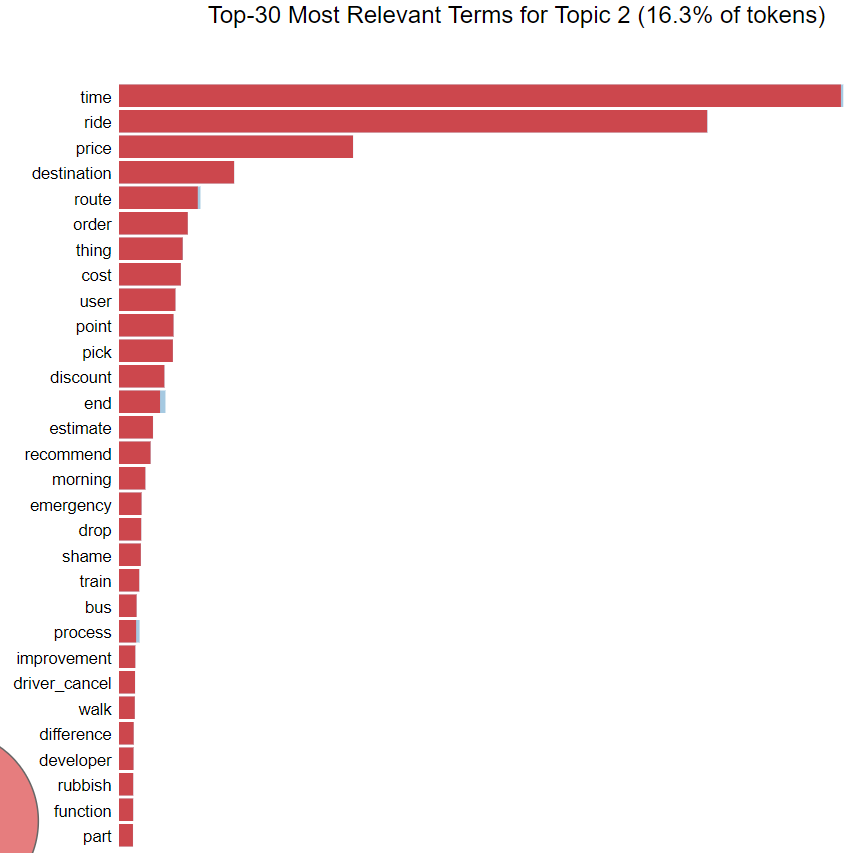
\includegraphics[width=0.7\textwidth]{figures/topic_ride_time.png}
    \caption{Extracted Keywords From Topic Ride Time}
    \label{fig:my_label}
\end{figure}

\begin{figure}[h]
    \centering
    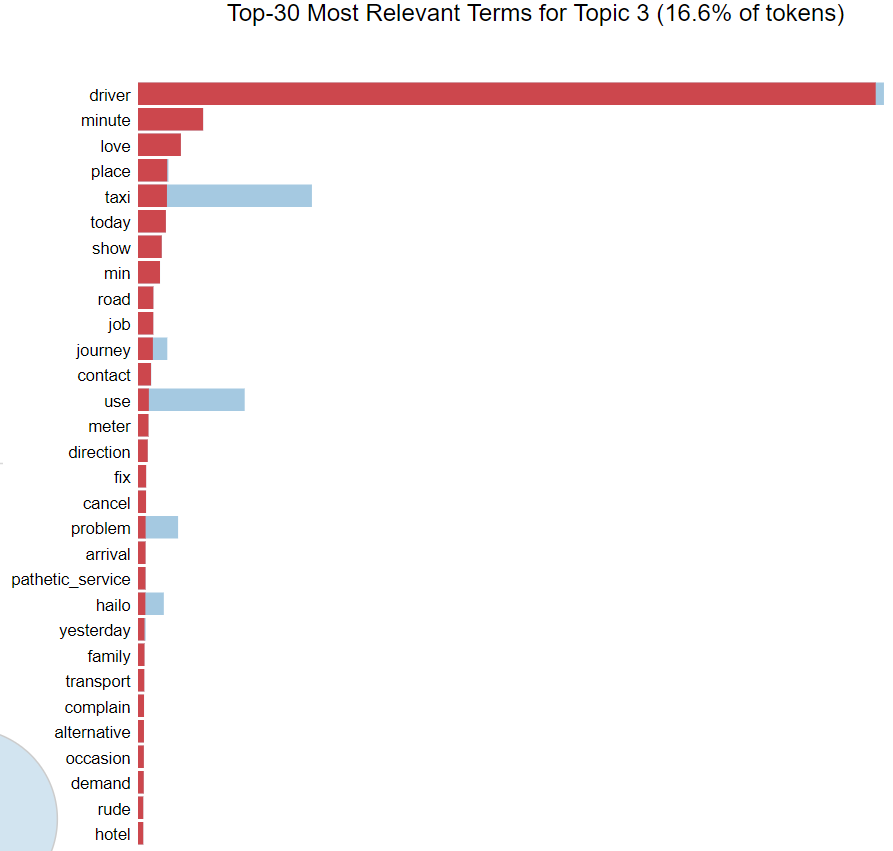
\includegraphics[width=0.65\textwidth]{figures/topic_driver_quality.png}
    \caption{Extracted Keywords From Topic Driver Quality}
    \label{fig:my_label}
\end{figure}

\begin{figure}[h]
    \centering
    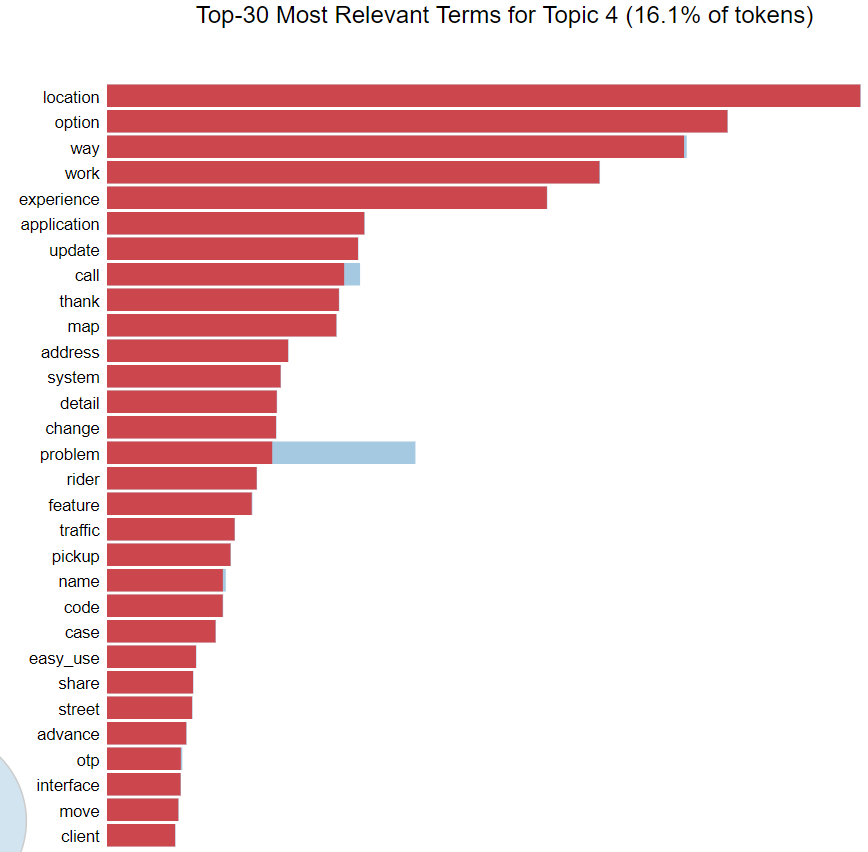
\includegraphics[width=0.65\textwidth]{figures/topic_location.png}
    \caption{Extracted Keywords From Topic Location}
    \label{fig:my_label}
\end{figure}

\begin{figure}[h]
    \centering
    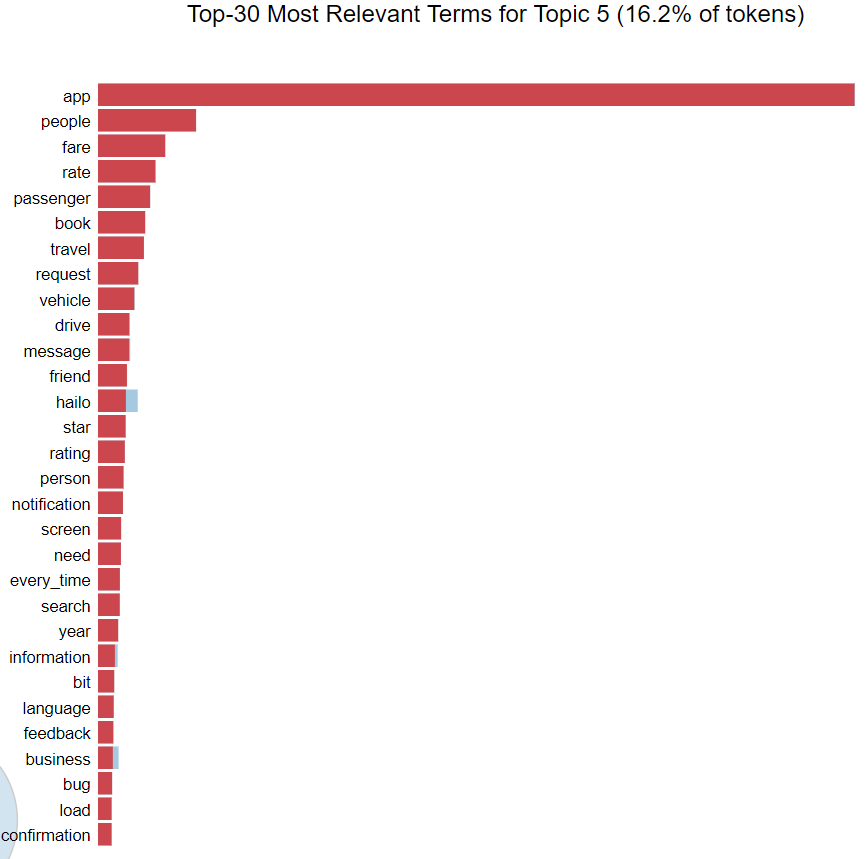
\includegraphics[width=0.62\textwidth]{figures/topic_app_experience.png}
    \caption{Extracted Keywords From Topic App Experience}
    \label{fig:my_label}
\end{figure}

\begin{figure}[h]
    \centering
    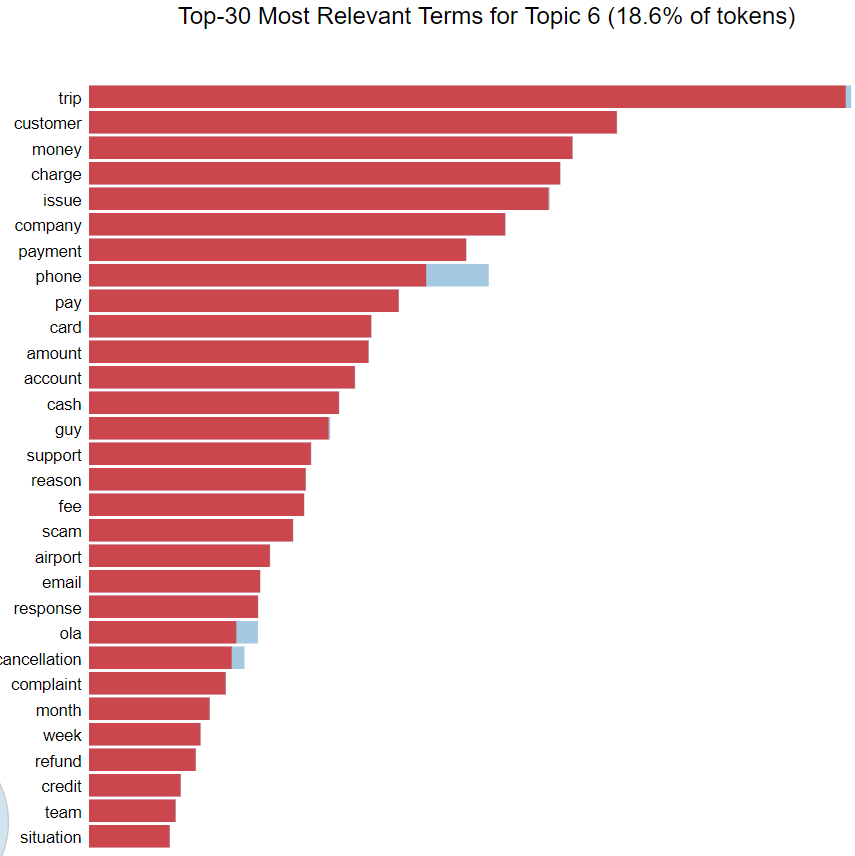
\includegraphics[width=0.62\textwidth]{figures/topic_trip_exp.png}
    \caption{Extracted Keywords From Topic Trip Experience}
    \label{fig:my_label}
\end{figure}

\newpage
\clearpage
%=== Licence in English
\newcommand{\licencehint}[2]{\\\hspace*{#1}\textsl(#2)\par}
\newcommand\EngLicence{{%
\selectlanguage{english}
\newpage
\section*{IV. Licence}

\addcontentsline{toc}{subsection}{IV. Licence}
\subsection*{Non-exclusive licence to reproduce thesis and make thesis public}

I, \textbf{Enlik -}, %author's name

\begin{enumerate}
\item
herewith grant the University of Tartu a free permit (non-exclusive licence) to
\par
reproduce, for the purpose of preservation, including for adding to the DSpace digital archives until the expiry of the term of copyright,
\par
\textbf{Topic Modeling for Requirements Engineering: An Analysis of Ridesharing App Reviews},
\par
supervised by Tahira Iqbal and Kuldar Taveter, PhD. %supervisor's name
\item
I grant the University of Tartu a permit to make the work specified in p. 1 available to the public via the web environment of the University of Tartu, including via the DSpace digital archives, under the Creative Commons licence CC BY NC ND 3.0, which allows, by giving appropriate credit to the author, to reproduce, distribute the work and communicate it to the public, and prohibits the creation of derivative works and any commercial use of the work until the expiry of the term of copyright.
\item
I am aware of the fact that the author retains the rights specified in p. 1 and 2.
\item
I certify that granting the non-exclusive licence does not infringe other persons' intellectual property rights or rights arising from the personal data protection legislation. 
\end{enumerate}

\noindent
Enlik -\\ %author's name
\textbf{\textsl{05/08/2022}}
}}%\newcommand\EngLicence


%=== Licence in Estonian
\newcommand\EstLicence{{%
\selectlanguage{estonian}
\section*{IV. Litsents}

\addcontentsline{toc}{subsection}{IV. Litsents}

\subsection*{Lihtlitsents lõputöö reprodutseerimiseks ja üldsusele kättesaadavaks tegemiseks}

Mina, \textbf{Alice Cooper}, %author's name
  \licencehint{10mm}{autori nimi}

\begin{enumerate}
\item
annan Tartu Ülikoolile tasuta loa (lihtlitsentsi) minu loodud teose
\par
\textbf{Tüübituletus neljandat järku loogikavalemitele}, %title of thesis
    \licencehint{10mm}{lõputöö pealkiri}
\par
mille juhendaja(d) on Axel Rose ja May Flower, %supervisor's name(s)
  \licencehint{10mm}{juhendaja nimi}
\par
reprodutseerimiseks eesmärgiga seda säilitada, sealhulgas lisada digitaalarhiivi DSpace kuni autoriõiguse kehtivuse lõppemiseni.
\par
\item
Annan Tartu Ülikoolile loa teha punktis 1 nimetatud teos üldsusele kättesaadavaks Tartu Ülikooli veebikeskkonna, sealhulgas digitaalarhiivi DSpace kaudu Creative Commonsi litsentsiga CC BY NC ND 3.0, mis lubab autorile viidates teost reprodutseerida, levitada ja üldsusele suunata ning keelab luua tuletatud teost ja kasutada teost ärieesmärgil, kuni autoriõiguse kehtivuse lõppemiseni.
\item
Olen teadlik, et punktides 1 ja 2 nimetatud õigused jäävad alles ka autorile.
\item
Kinnitan, et lihtlitsentsi andmisega ei riku ma teiste isikute intellektuaalomandi ega isikuandmete kaitse õigusaktidest tulenevaid õigusi. 
\end{enumerate}

\noindent
Enlik\\ %author's name
\textbf{\textsl{pp.kk.aaaa}}
}}%\newcommand\EstLicence


%===Choose the licence in active language
\iflanguage{english}{\EngLicence}{\EstLicence}


\end{document}